Se ha desarrollado un conjunto de bocetos representativos para cada una de las interfaces principales, con el objetivo de facilitar la comprensión visual y estructural del sistema. 
Se ha decidido omitir la creación de bocetos para ciertas páginas del sistema, considerando que su simplicidad inherente no justifica una representación gráfica detallada, 
o debido a que su diseño es análogo al de otras interfaces previamente especificadas. 

\subsubsection{Página de Inicio}
La página de inicio es la primera página que se muestra al usuario al acceder al sistema.
Esta página se muestra cuando el usuario no ha iniciado sesión, y le permite acceder a las siguientes funcionalidades:
\begin{itemize}
    \item Iniciar sesión.
    \item Registrarse.
    \item Consultar información pública sobre el sistema (Enlaces del pie de página)
\end{itemize}

En la \coloredUnderline{\hyperlink{fig:p_home}{Figura \ref*{fig:p_homes}: \nameref*{fig:p_home}}} se muestra el boceto de la página de inicio.

\begin{figure}[H]
    \centering
    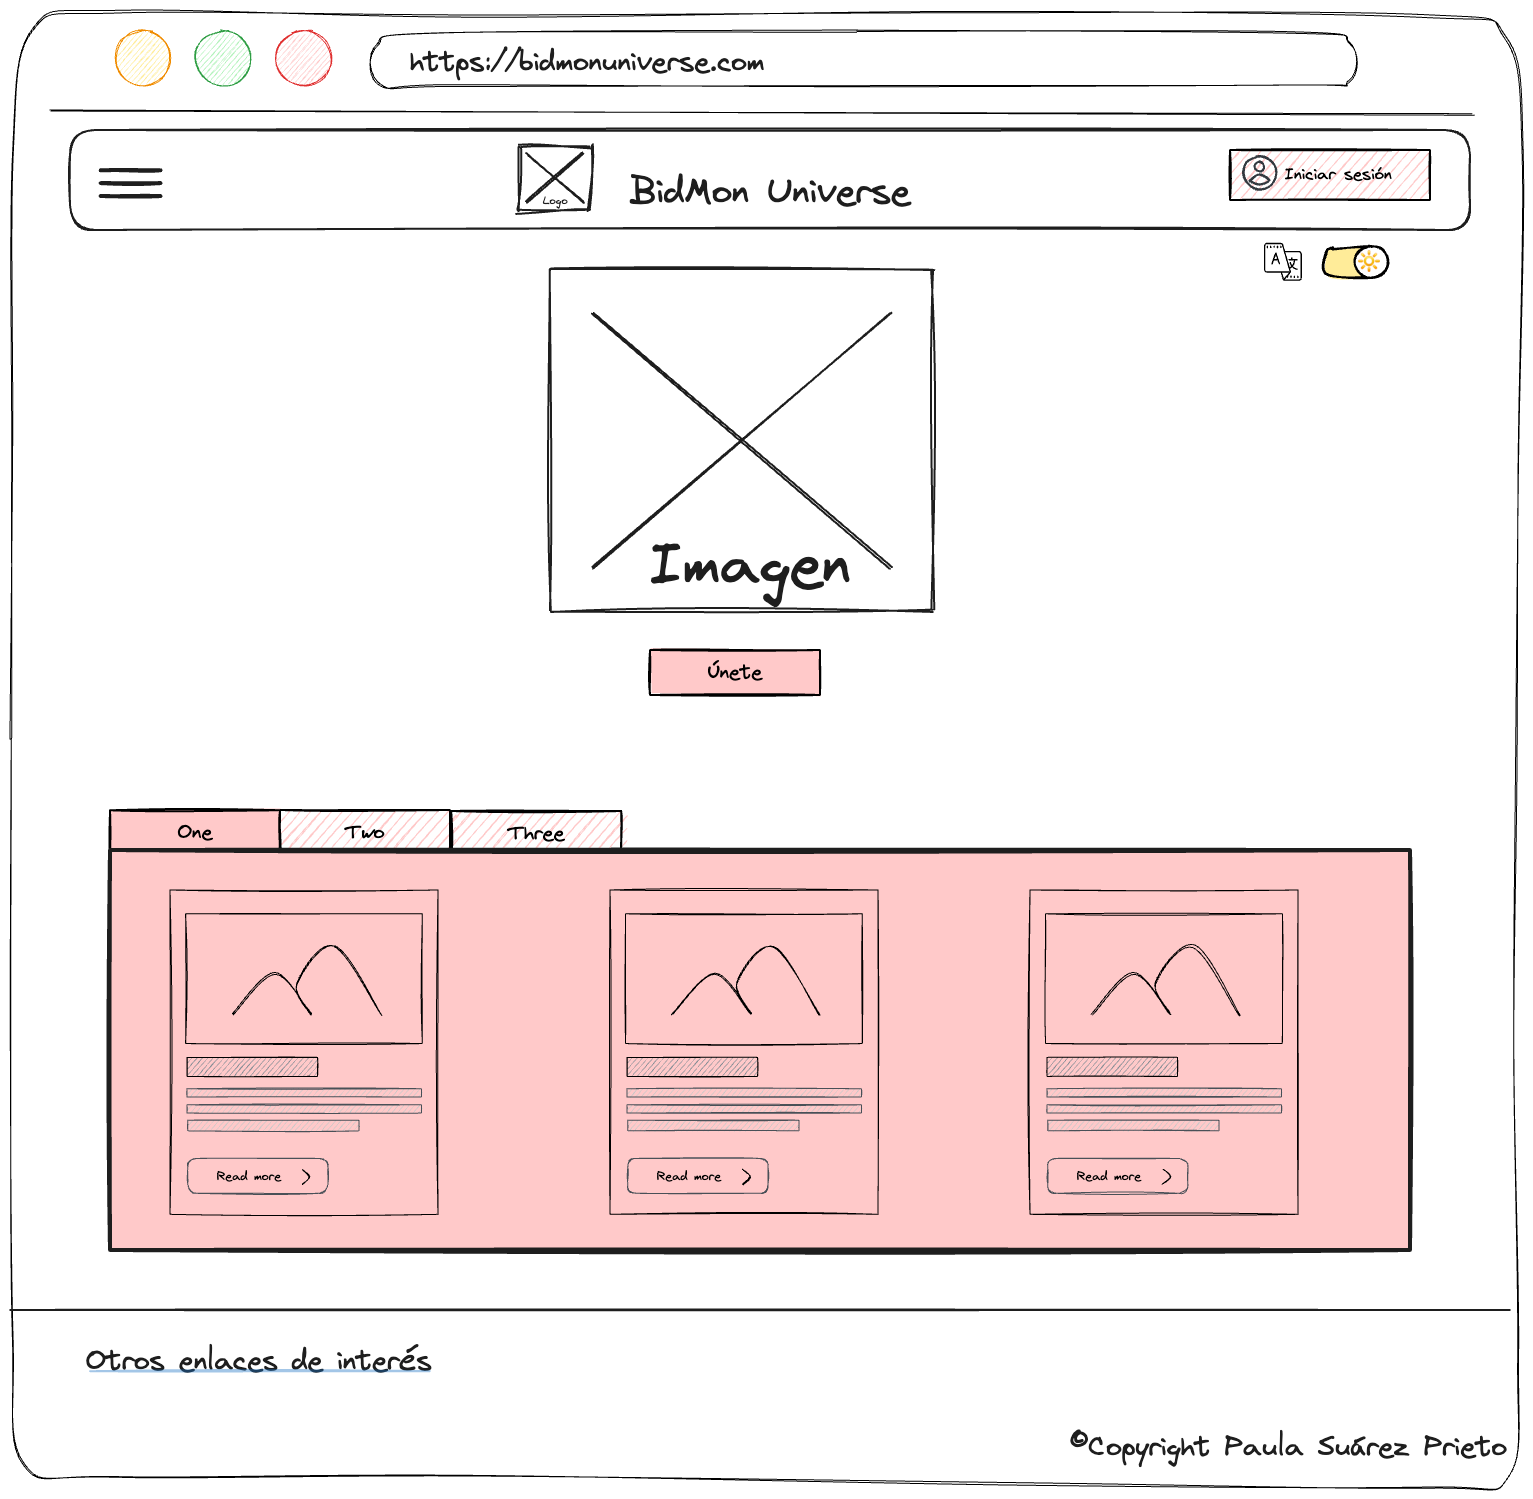
\includegraphics[width=0.8\textwidth]{figures/6-Analisis/6-Interfaz/prototipos/home.png}
    \caption{Boceto de la página de inicio}
    \label{fig:p_home}
    \hypertarget{fig:p_home}{}
\end{figure}

\subsubsection{Página de Inicio de Sesión}
La página de inicio de sesión muestra un formulario que permite al usuario ingresar sus credenciales para acceder al sistema o recuperar su contraseña.

En la \coloredUnderline{\hyperlink{fig:p_login}{Figura \ref*{fig:p_login}: \nameref*{fig:p_login}}} se muestra el boceto de la página de inicio de sesión.
En caso de que el usuario introduzca credenciales incorrectas, se mostrará un mensaje de error y se resaltarán los campos correspondientes.

\begin{figure}[H]
    \centering
    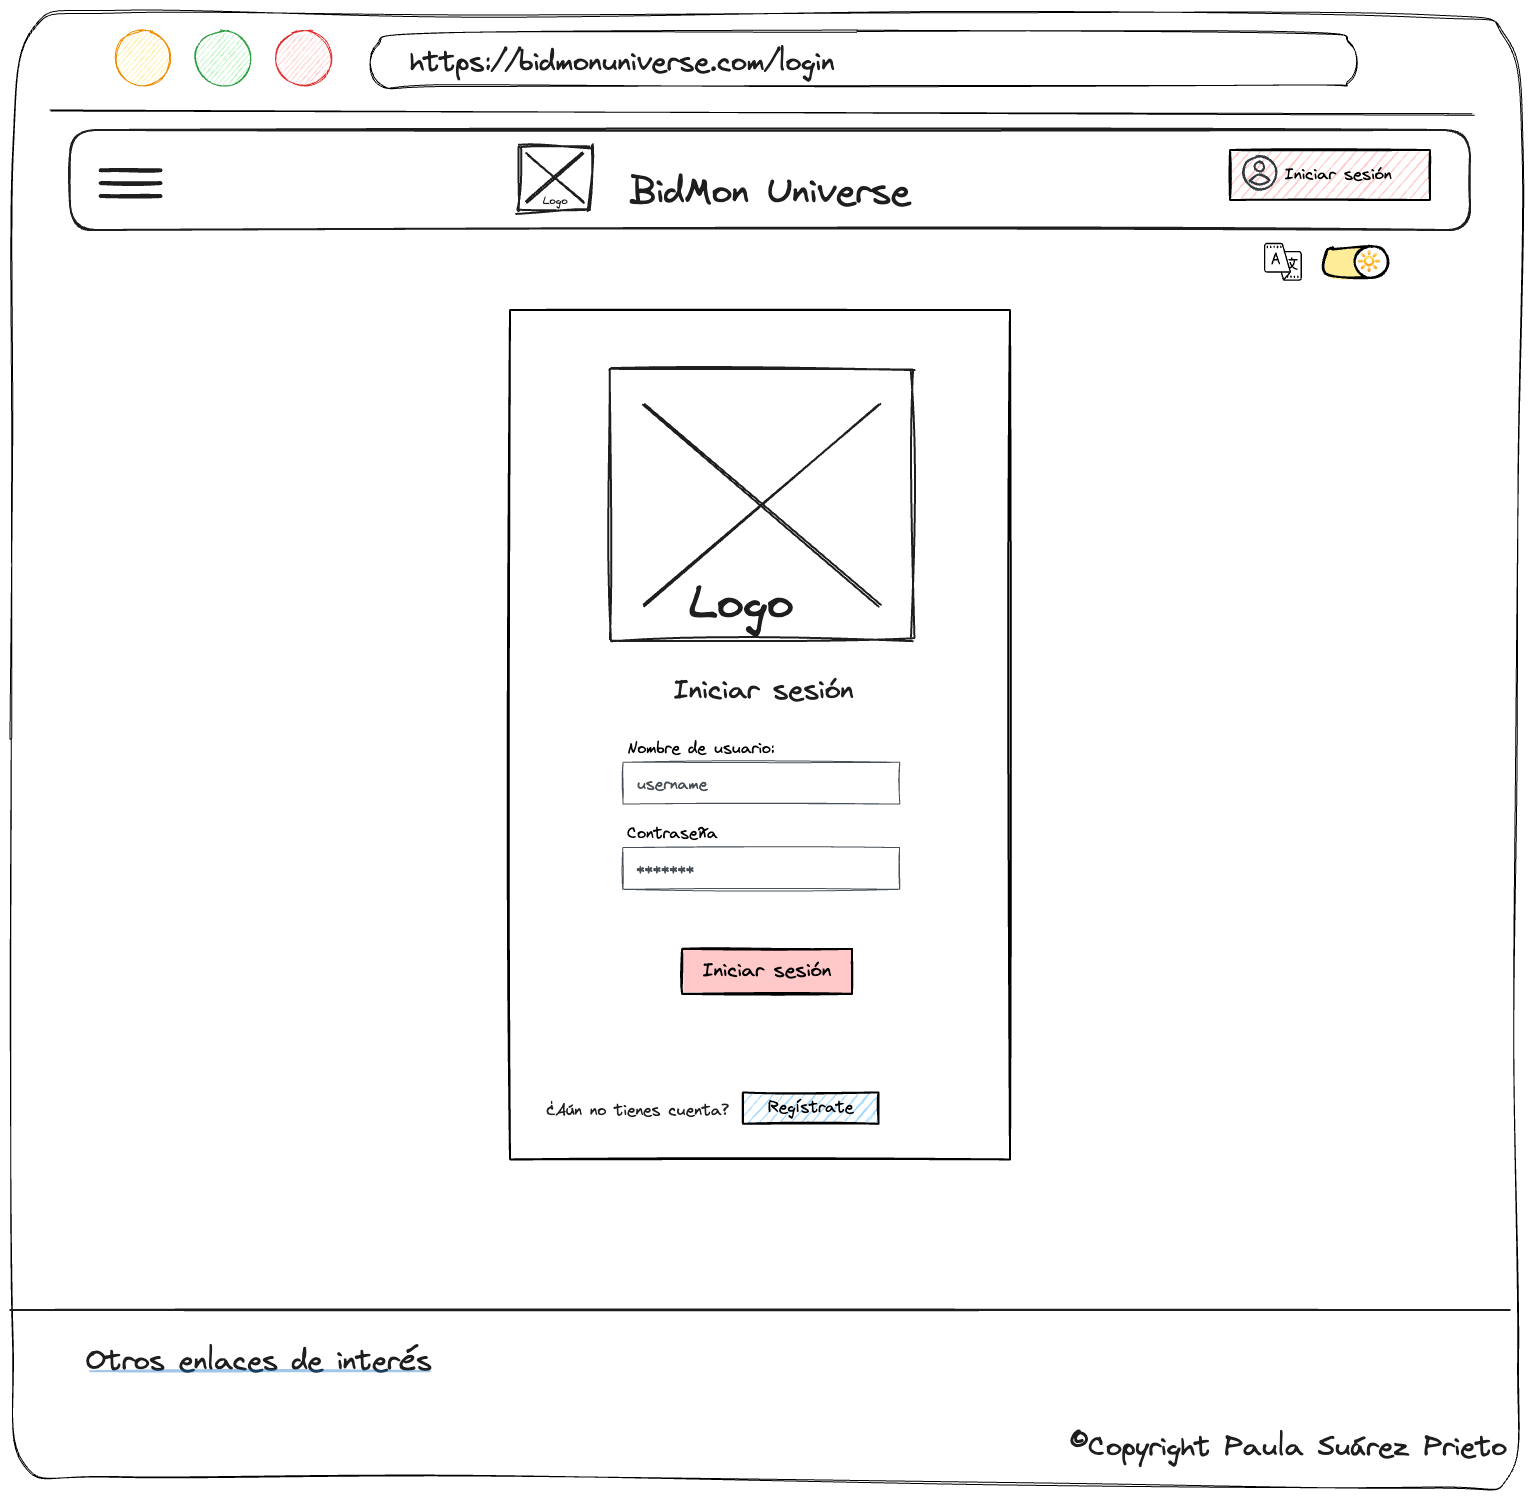
\includegraphics[width=0.8\textwidth]{figures/6-Analisis/6-Interfaz/prototipos/login.png}
    \caption{Boceto de la página de inicio de sesión}
    \label{fig:p_login}
    \hypertarget{fig:p_login}{}
\end{figure}

\subsubsection{Página de Registro}
La página de registro muestra un formulario que permite al usuario crear una cuenta en el sistema o iniciar sesión si ya tiene una cuenta.
En la \coloredUnderline{\hyperlink{fig:p_signup}{Figura \ref*{fig:p_signup}: \nameref*{fig:p_signup}}} se muestra el boceto de la página de registro.

En caso de que los campos del formulario no cumplan con las restricciones especificadas, se mostrará un mensaje de error y se resaltarán los campos correspondientes.

\begin{figure}[H]
    \centering
    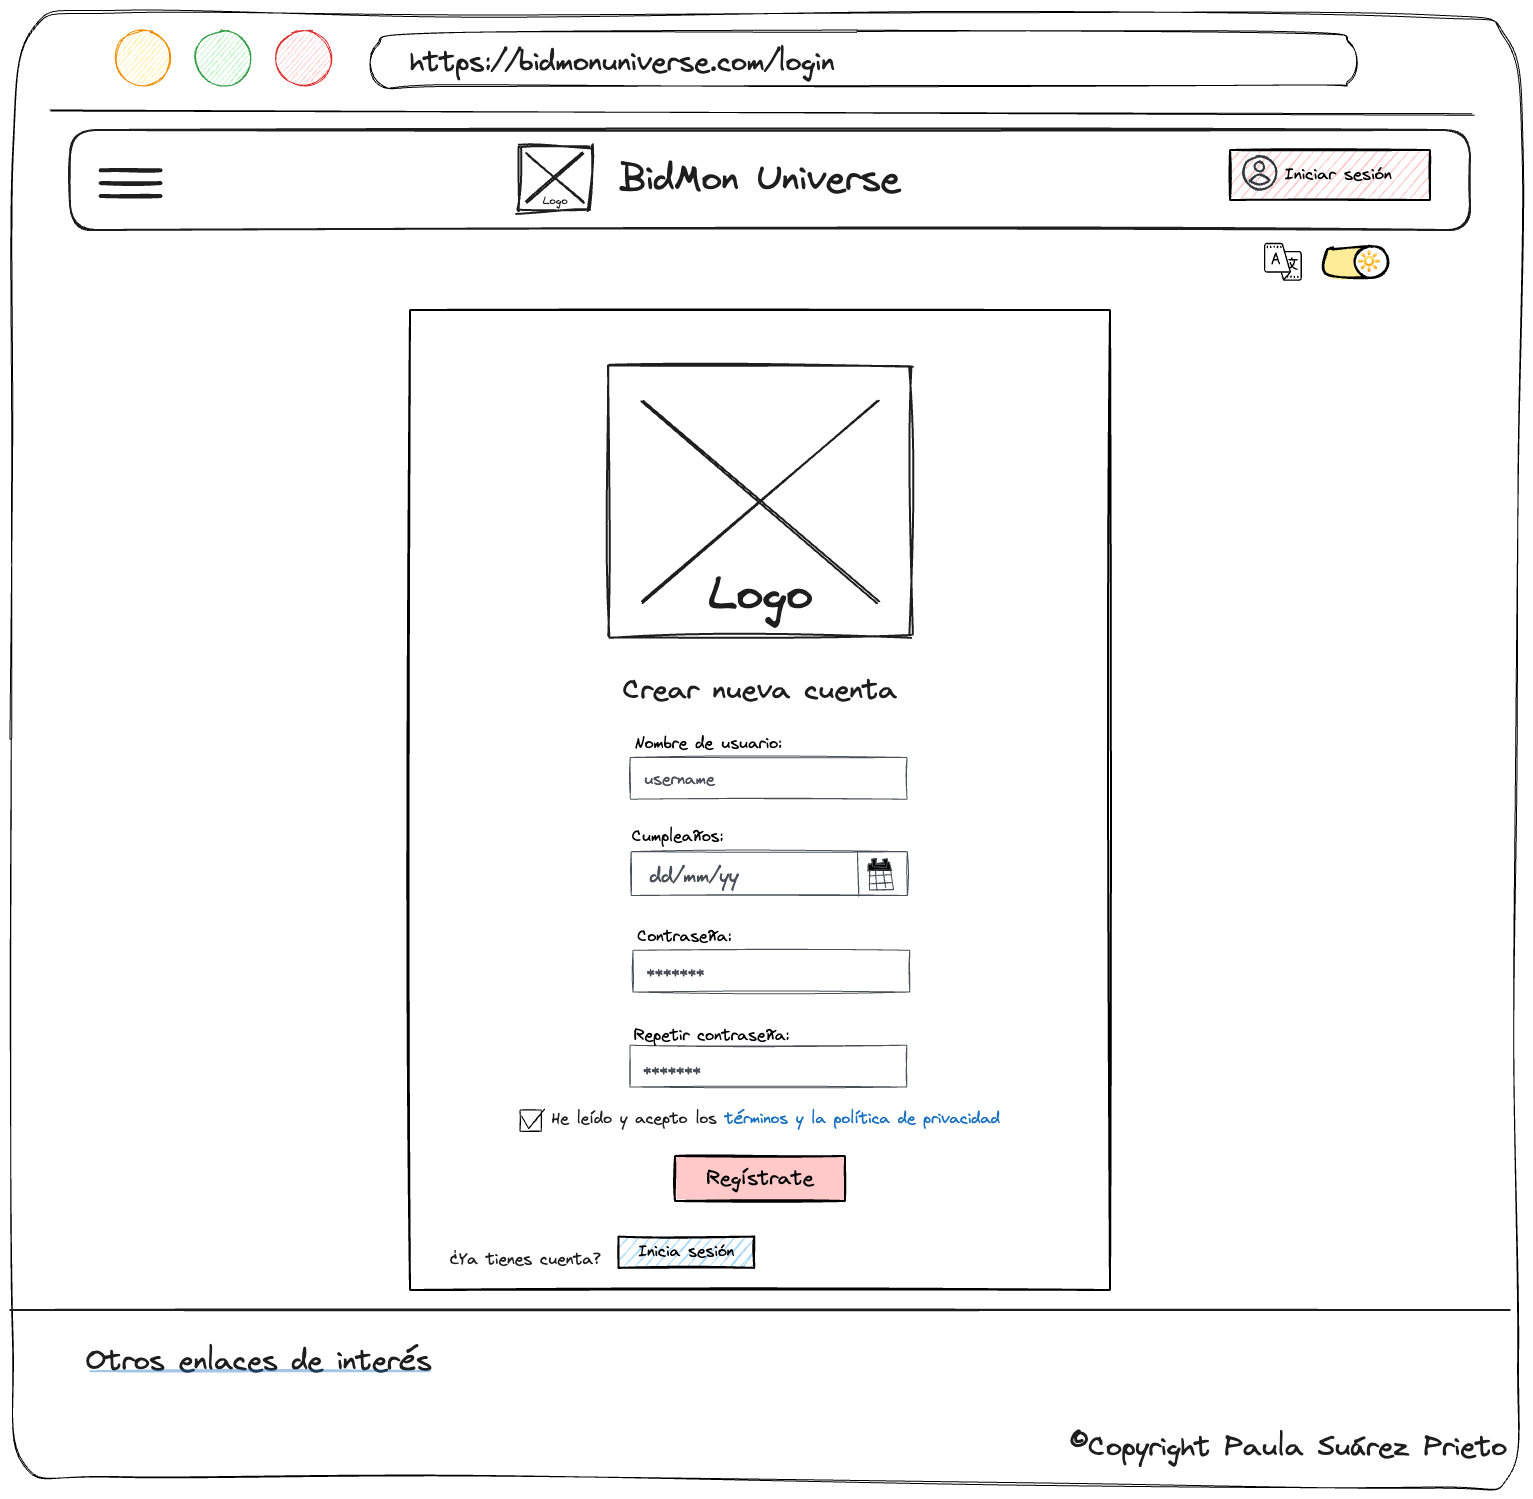
\includegraphics[width=0.8\textwidth]{figures/6-Analisis/6-Interfaz/prototipos/signup.png}
    \caption{Boceto de la página de registro}
    \label{fig:p_signup}
    \hypertarget{fig:p_signup}{}
\end{figure}

\subsubsection{Página inicial de usuario}
Una vez que el usuario ha iniciado sesión en la plataforma, se le redirige a la página inicial de usuario.
Las páginas a las que tiene acceso un usuario autenticado muestran siempre como cabecera de la página un menú general de navegación que le permite acceder a las diferentes secciones del sistema,
el saldo de su cuenta y un menú de usuario que le permite acceder a su perfil y cerrar sesión.

La página inicial de usuario muestra un resumen de la información más relevante para el usuario:
\begin{itemize}
    \item Menú de acceso rápido a las secciones principales del sistema.
    \item Muestra las cartas más recientes de su colección con la posibilidad de acceder a la colección completa.
    \item Muestra las subastas activas iniciadas por el usuario más recientes con la posibilidad de acceder a las subastas completas.
    \item Muestra las pujas activas más recientes realizadas por el usuario con la posibilidad de acceder a las pujas completas.
\end{itemize}

En la \coloredUnderline{\hyperlink{fig:p_user_home}{Figura \ref*{fig:p_user_home}: \nameref*{fig:p_user_home}}} se muestra el boceto de la página inicial de usuario.

\begin{figure}[H]
    \centering
    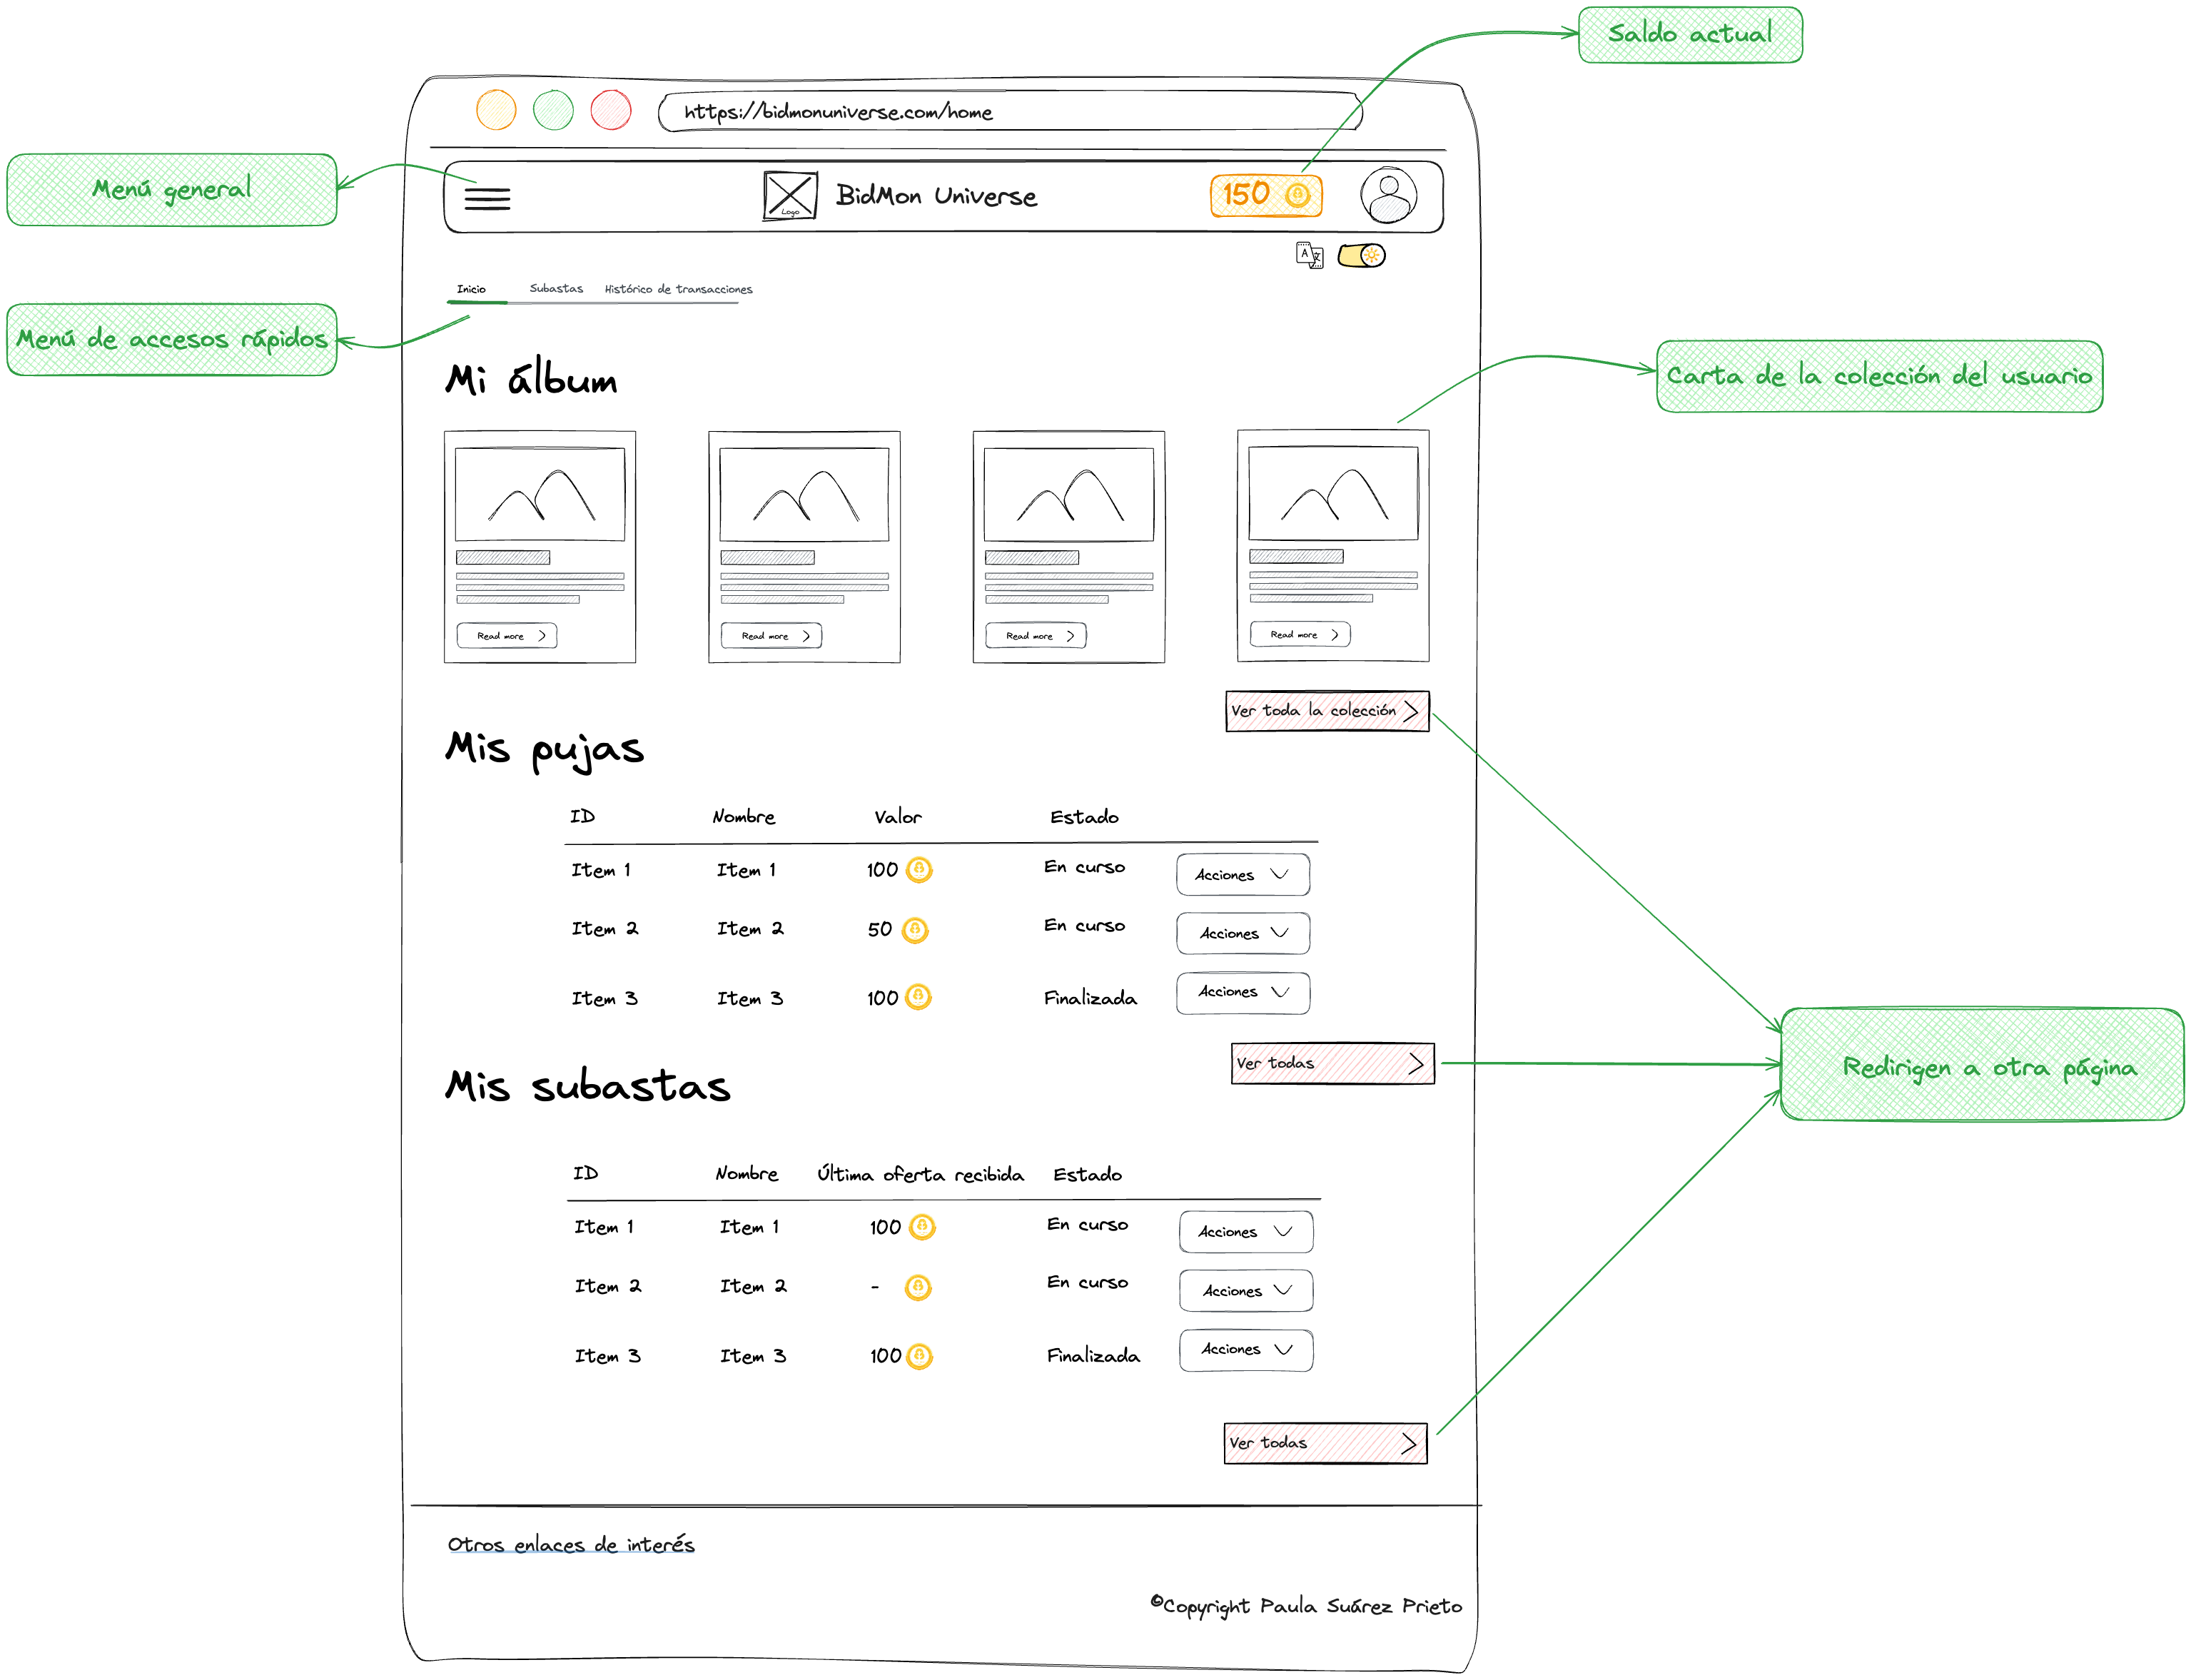
\includegraphics[width=1\textwidth]{figures/6-Analisis/6-Interfaz/prototipos/home-logueada.png}
    \caption{Boceto de la página inicial de usuario}
    \label{fig:p_user_home}
    \hypertarget{fig:p_user_home}{}
\end{figure}

\subsubsection{Página de Colección}
La página de colección muestra una lista de las cartas que el usuario ha añadido a su colección.
El usuario puede hacer clic en una carta para ver más detalles sobre ella.

En la \coloredUnderline{\hyperlink{fig:p_collection}{Figura \ref*{fig:p_collection}: \nameref*{fig:p_collection}}} se muestra el boceto de la página de colección.
\begin{figure}[H]
    \centering
    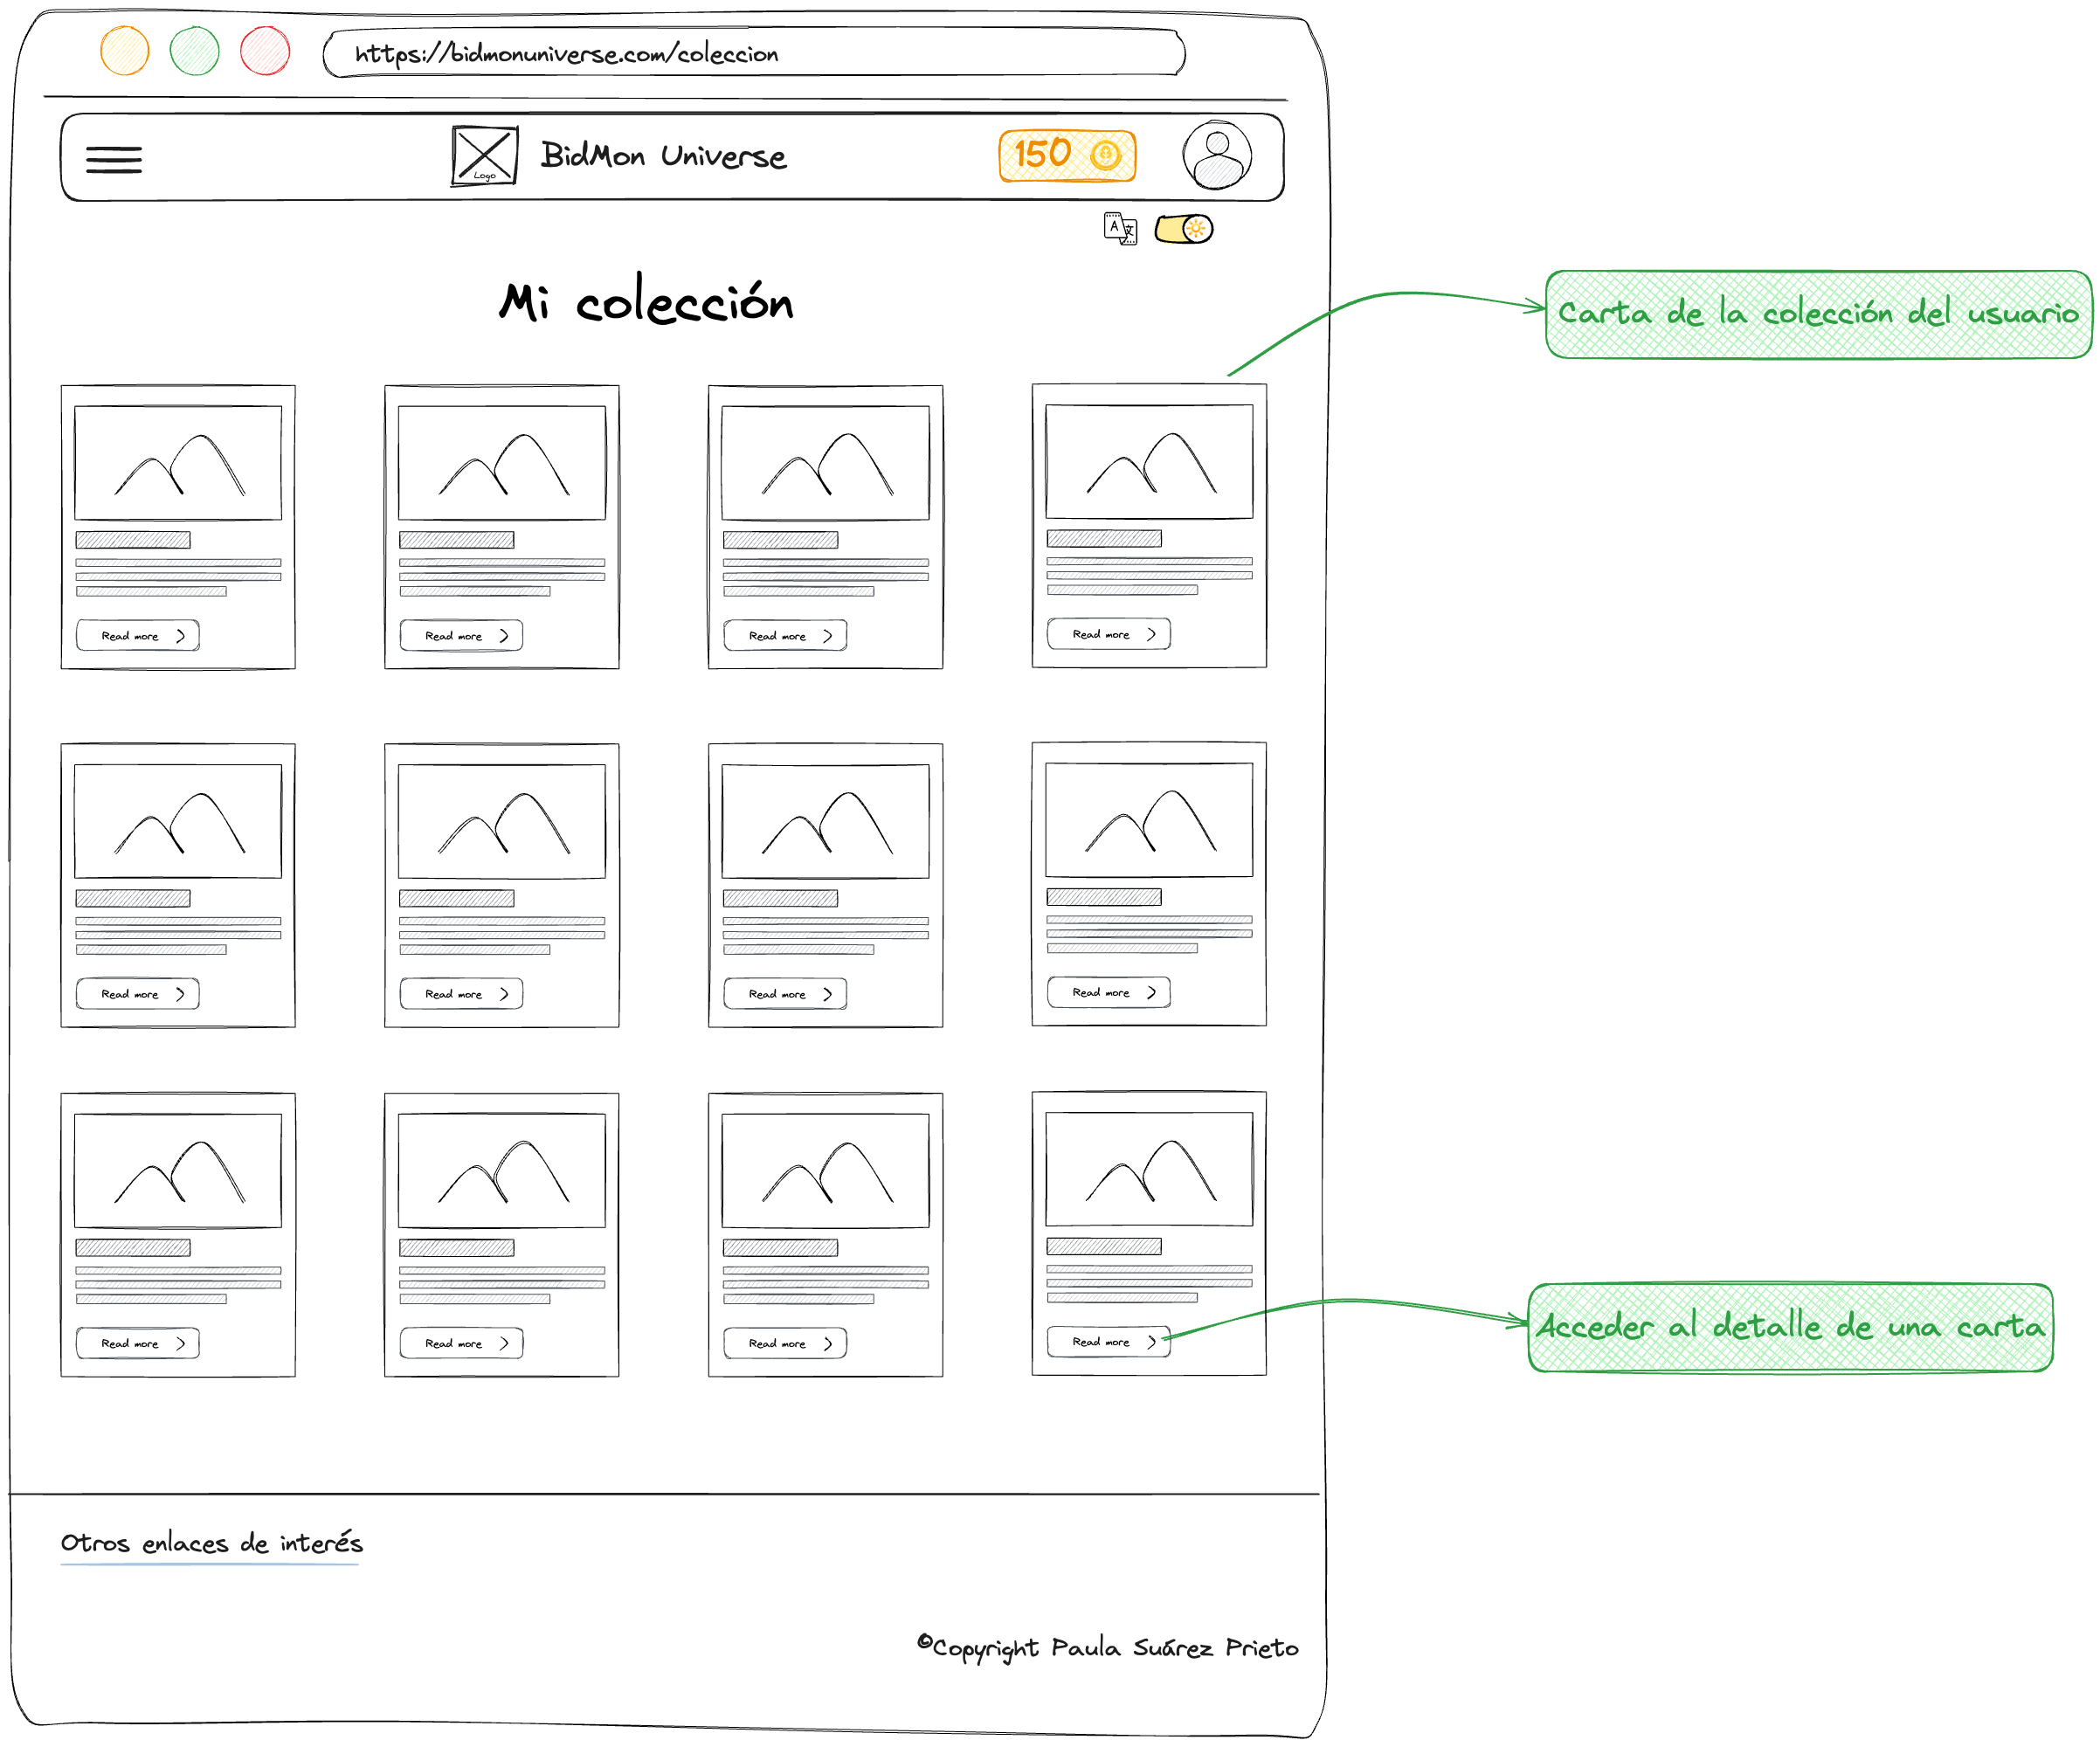
\includegraphics[width=0.9\textwidth]{figures/6-Analisis/6-Interfaz/prototipos/coleccion.png}
    \caption{Boceto de la página de colección}
    \label{fig:p_collection}
    \hypertarget{fig:p_collection}{}
\end{figure}

\subsubsection{Página de Detalles de Carta}
La página de detalles de carta muestra información detallada sobre una carta específica. Permite al usuario ver la imagen de la carta, los datos de la carta, 
las transacciones de esta y la posibilidad de marcar la carta como destacada o subastarla.

En la \coloredUnderline{\hyperlink{fig:p_card_details}{Figura \ref*{fig:p_card_details}: \nameref*{fig:p_card_details}}} se muestra el boceto de la página de detalles de carta.
\begin{figure}[H]
    \centering
    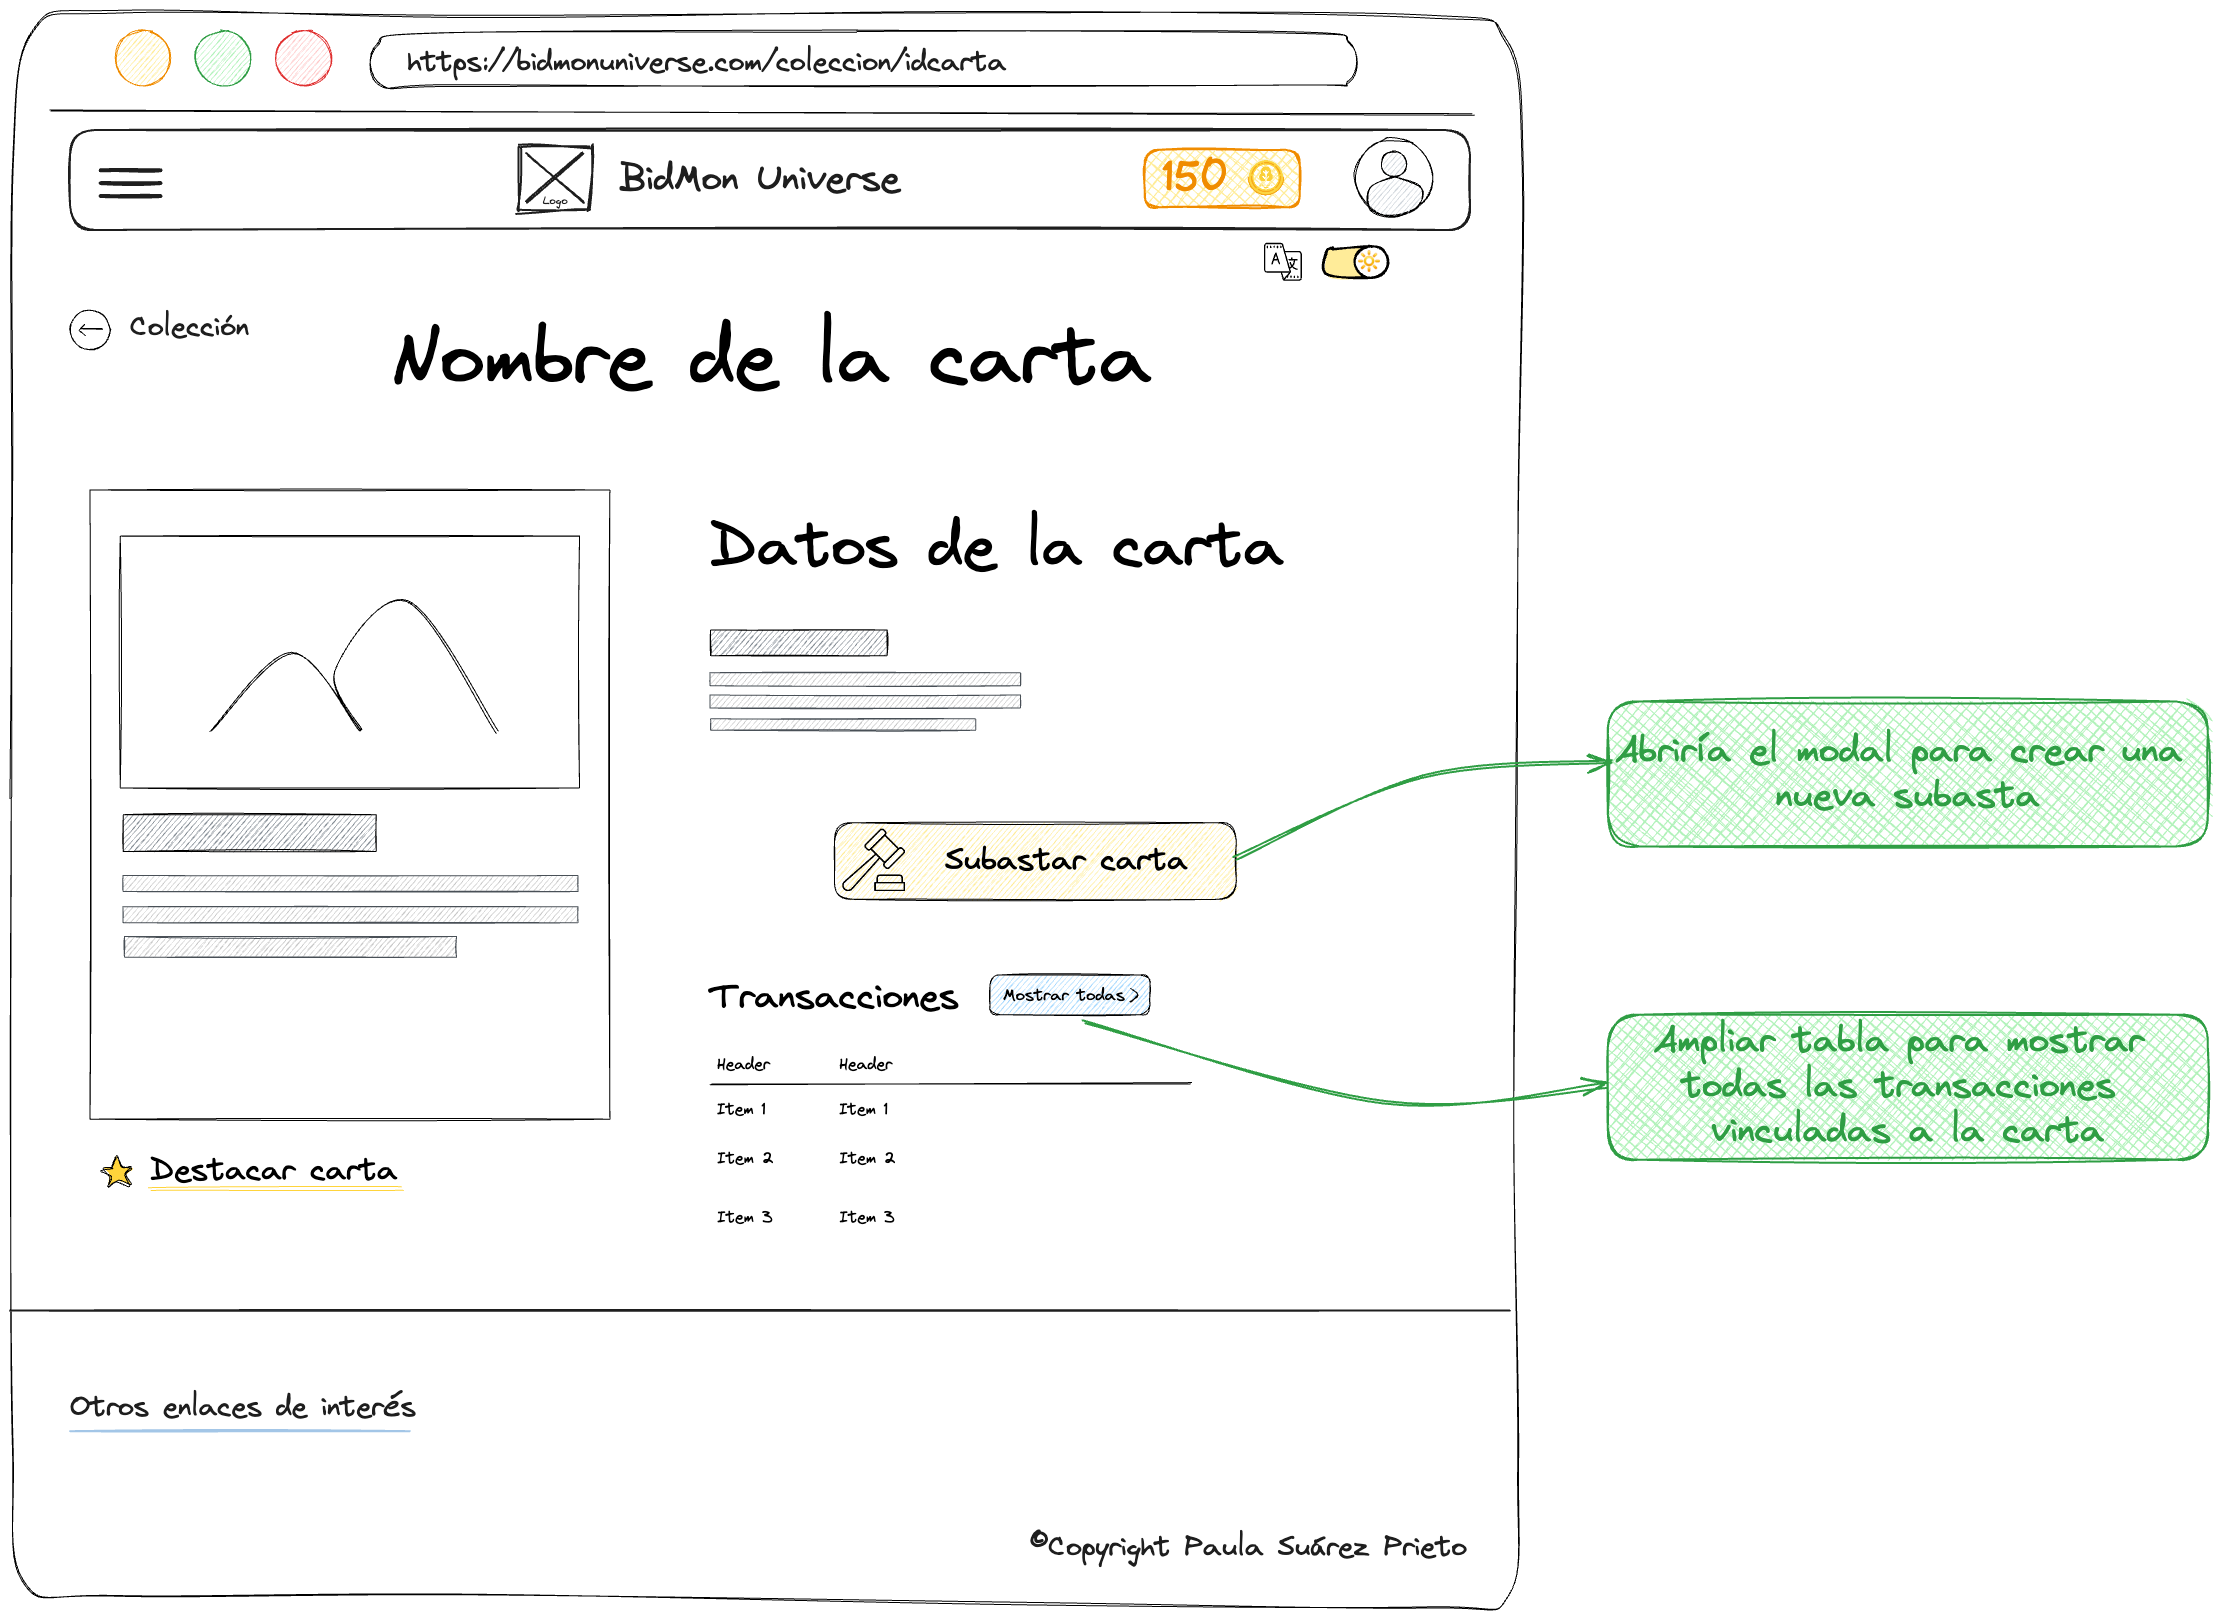
\includegraphics[width=0.9\textwidth]{figures/6-Analisis/6-Interfaz/prototipos/detalle-carta.png}
    \caption{Boceto de la página de detalles de carta}
    \label{fig:p_card_details}
    \hypertarget{fig:p_card_details}{}
\end{figure}

\subsubsection{Página de Creación de Subasta}
La página de creación de subasta muestra el detalle de la carta que se va a subastar y permite al usuario establecer el precio de salida y la duración de la subasta.
Estos valores deben cumplir con las restricciones especificadas y son opcionales, si el usuario no los establece se usarán los valores por defecto y se le informará en la ventana de confirmación.

En la \coloredUnderline{\hyperlink{fig:p_create_auction}{Figura \ref*{fig:p_create_auction}: \nameref*{fig:p_create_auction}}}, se muestra el boceto de la página de creación de subasta.
\begin{figure}[H]
    \centering
    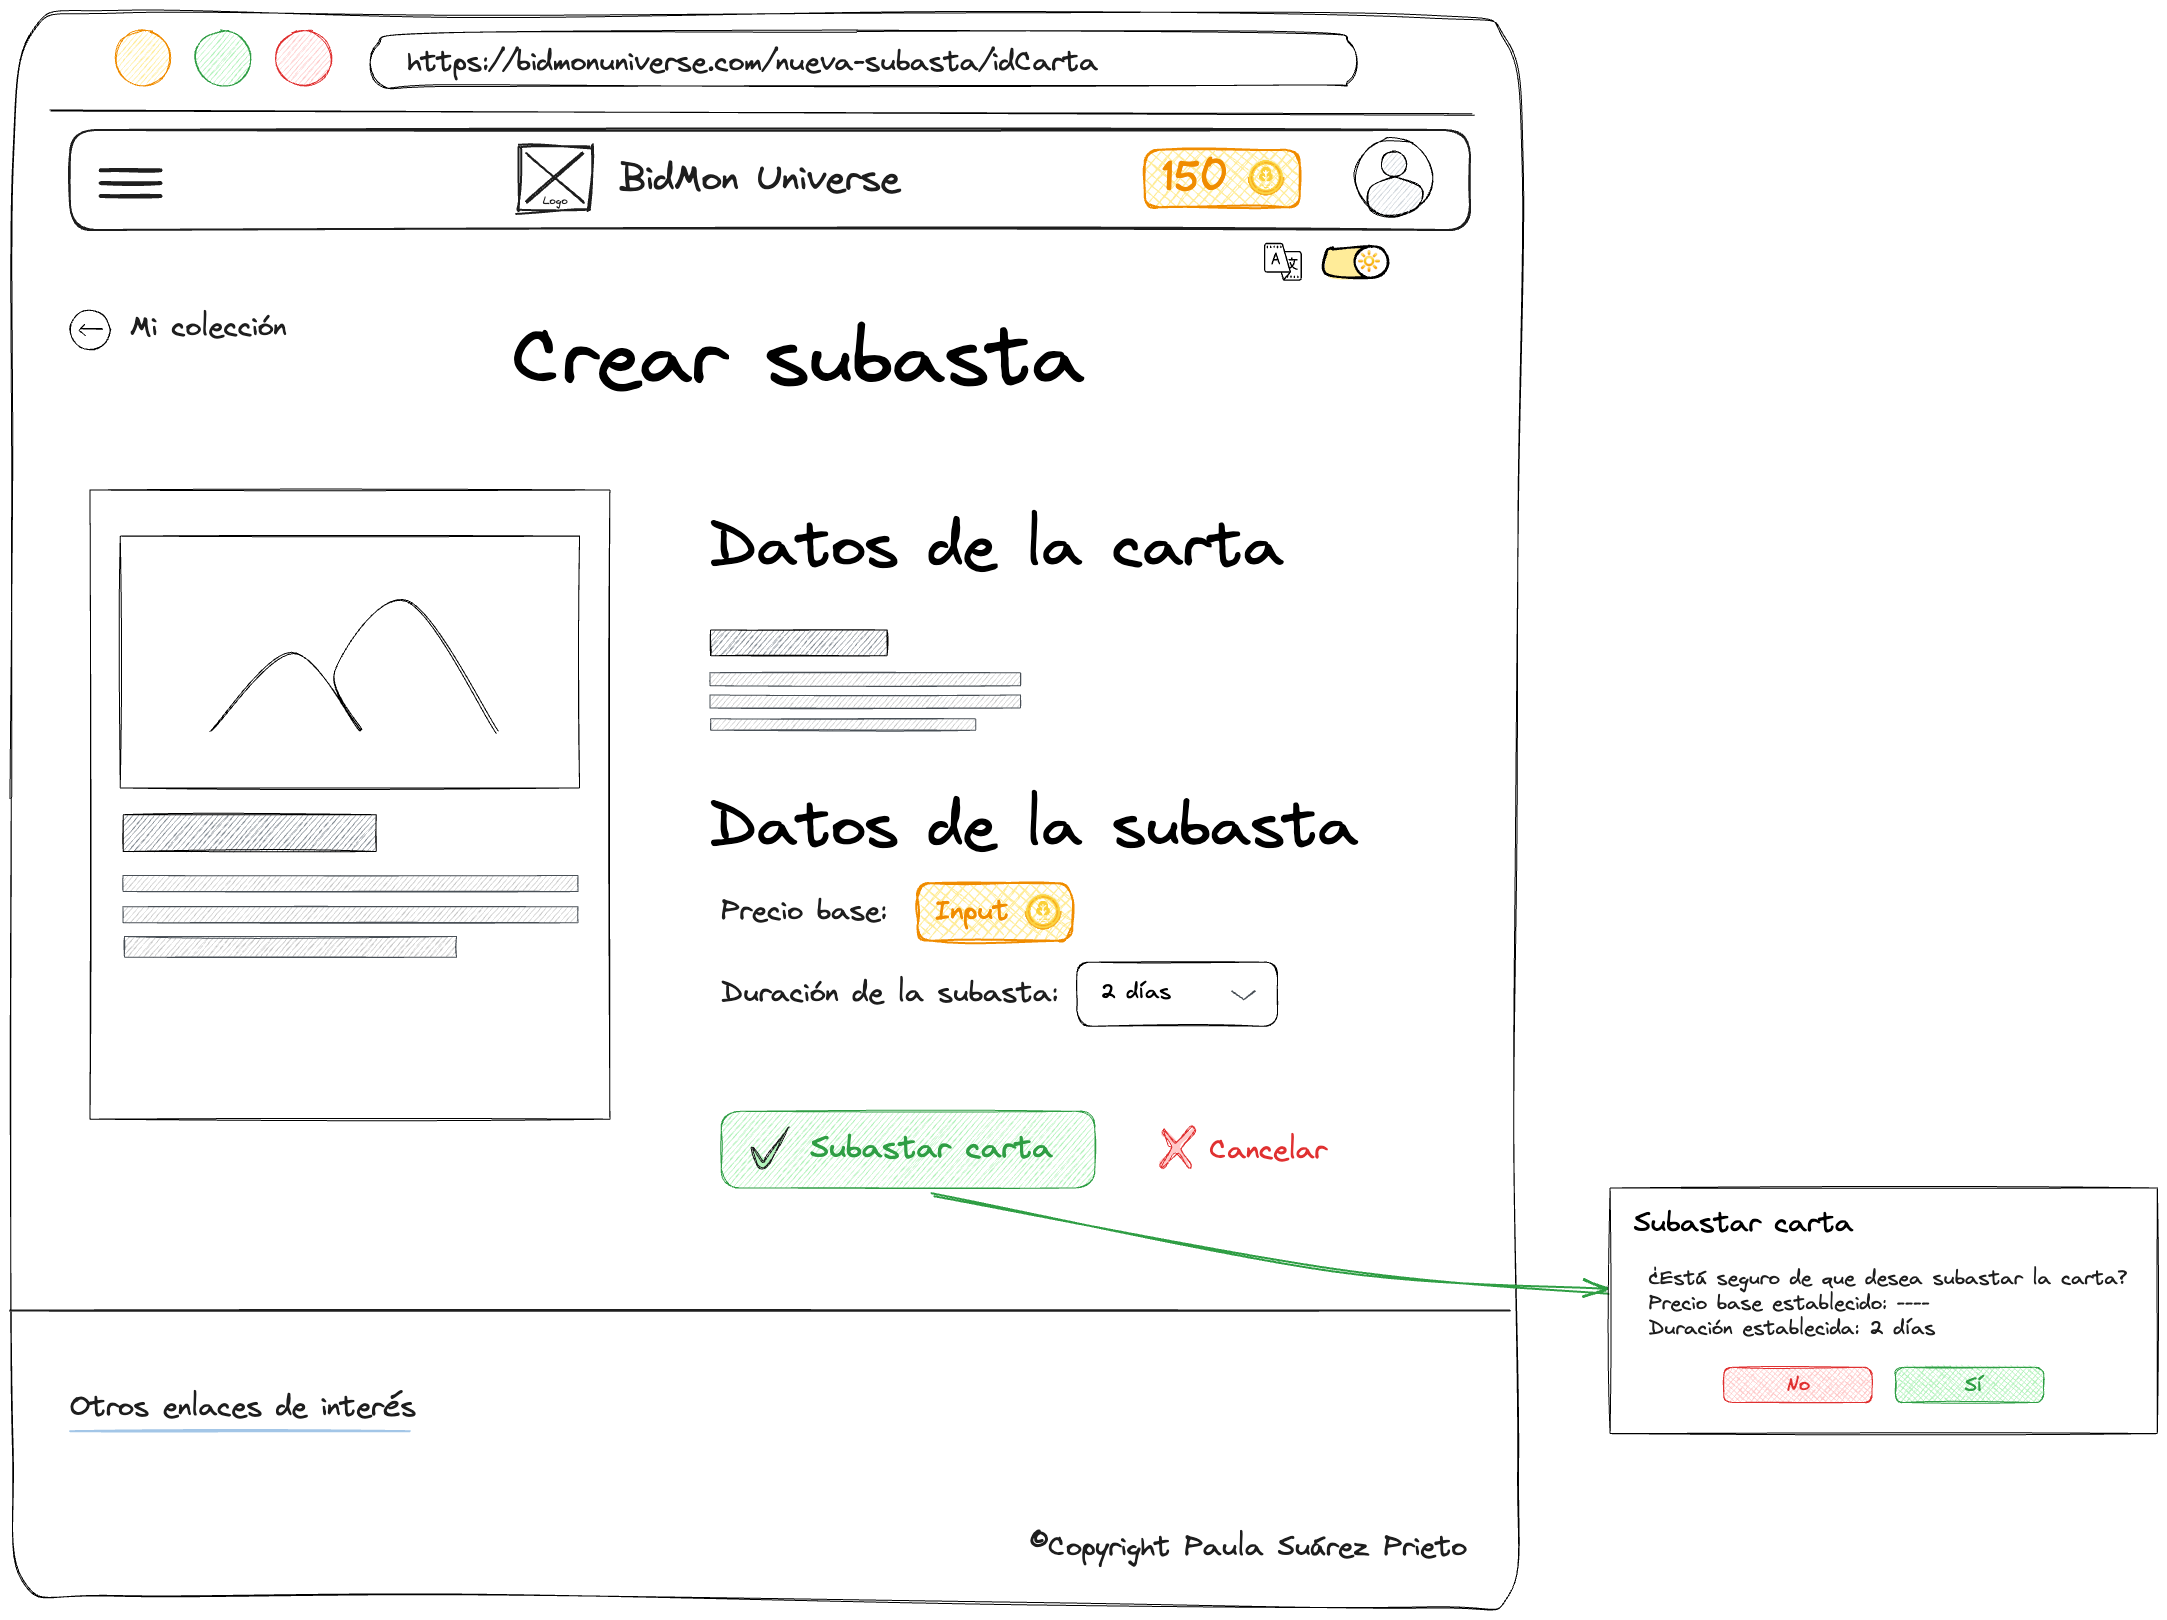
\includegraphics[width=0.9\textwidth]{figures/6-Analisis/6-Interfaz/prototipos/crear-subasta.png}
    \caption{Boceto de la página de creación de subasta}
    \label{fig:p_create_auction}
    \hypertarget{fig:p_create_auction}{}
\end{figure}


\subsubsection{Página de Subastas}
La página de subastas muestra una lista de las subastas activas en las que el usuario puede participar.
En esta página hay un menú de navegación que permite al usuario filtrar las subastas por diferentes criterios:
\begin{itemize}
    \item Todas: Todas las subastas activas.
    \item Mis Subastas: Subastas en las que el usuario ha creado.
    \item Pujas: Subastas en las que el usuario ha pujado.
\end{itemize}

La página de subastas muestra las cartas subastadas, al hacer clic en una carta se muestra la información detallada de la subasta.

En la \coloredUnderline{\hyperlink{fig:p_auctions}{Figura \ref*{fig:p_auctions}: \nameref*{fig:p_auctions}}}, se muestra el boceto de la página de subastas.
\begin{figure}[H]
    \centering
    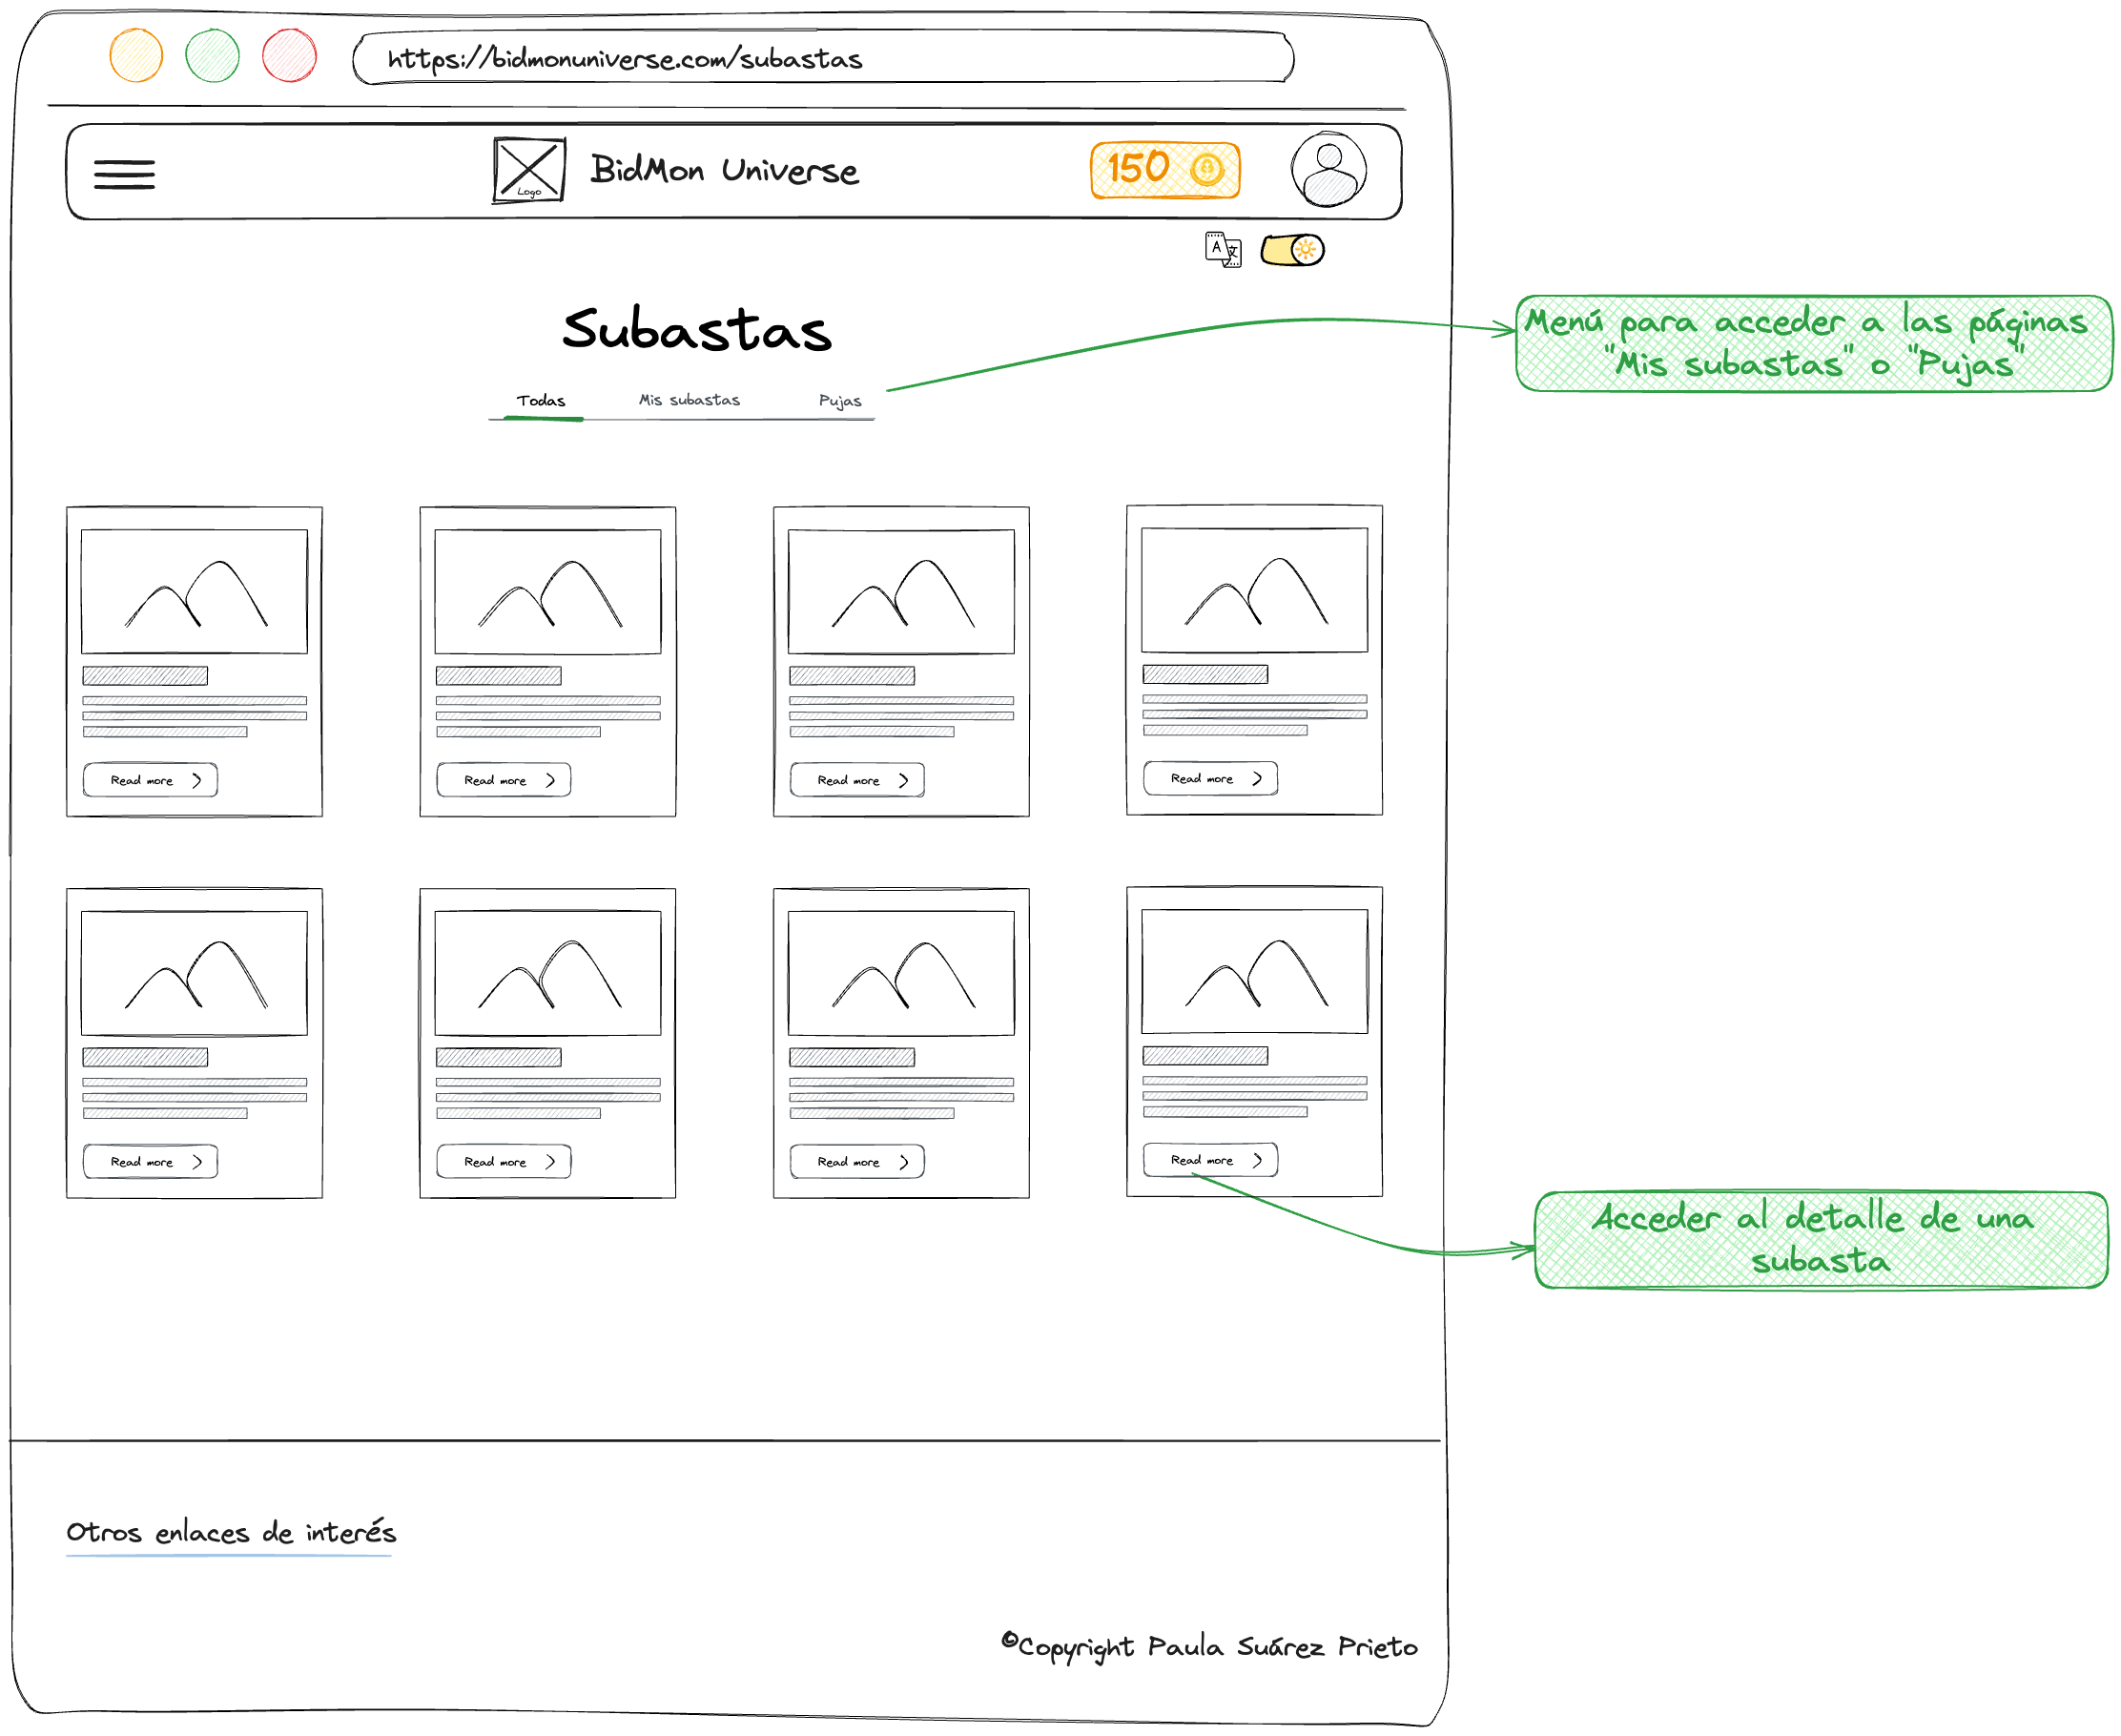
\includegraphics[width=0.9\textwidth]{figures/6-Analisis/6-Interfaz/prototipos/subastas.png}
    \caption{Boceto de la página de subastas}
    \label{fig:p_auctions}
    \hypertarget{fig:p_auctions}{}
\end{figure}

\subsubsection{Página de Detalles de Subasta}
La página de detalles de subasta muestra información detallada sobre una subasta específica.
Dependiendo de si la subasta es propia o no, el usuario puede realizar diferentes acciones.

En la \coloredUnderline{\hyperlink{fig:p_auction_details}{Figura \ref*{fig:p_auction_details}: \nameref*{fig:p_auction_details}}},
se muestra el boceto de la página de detalles de una subasta activa creada por otro usuario.
\begin{figure}[H]
    \centering
    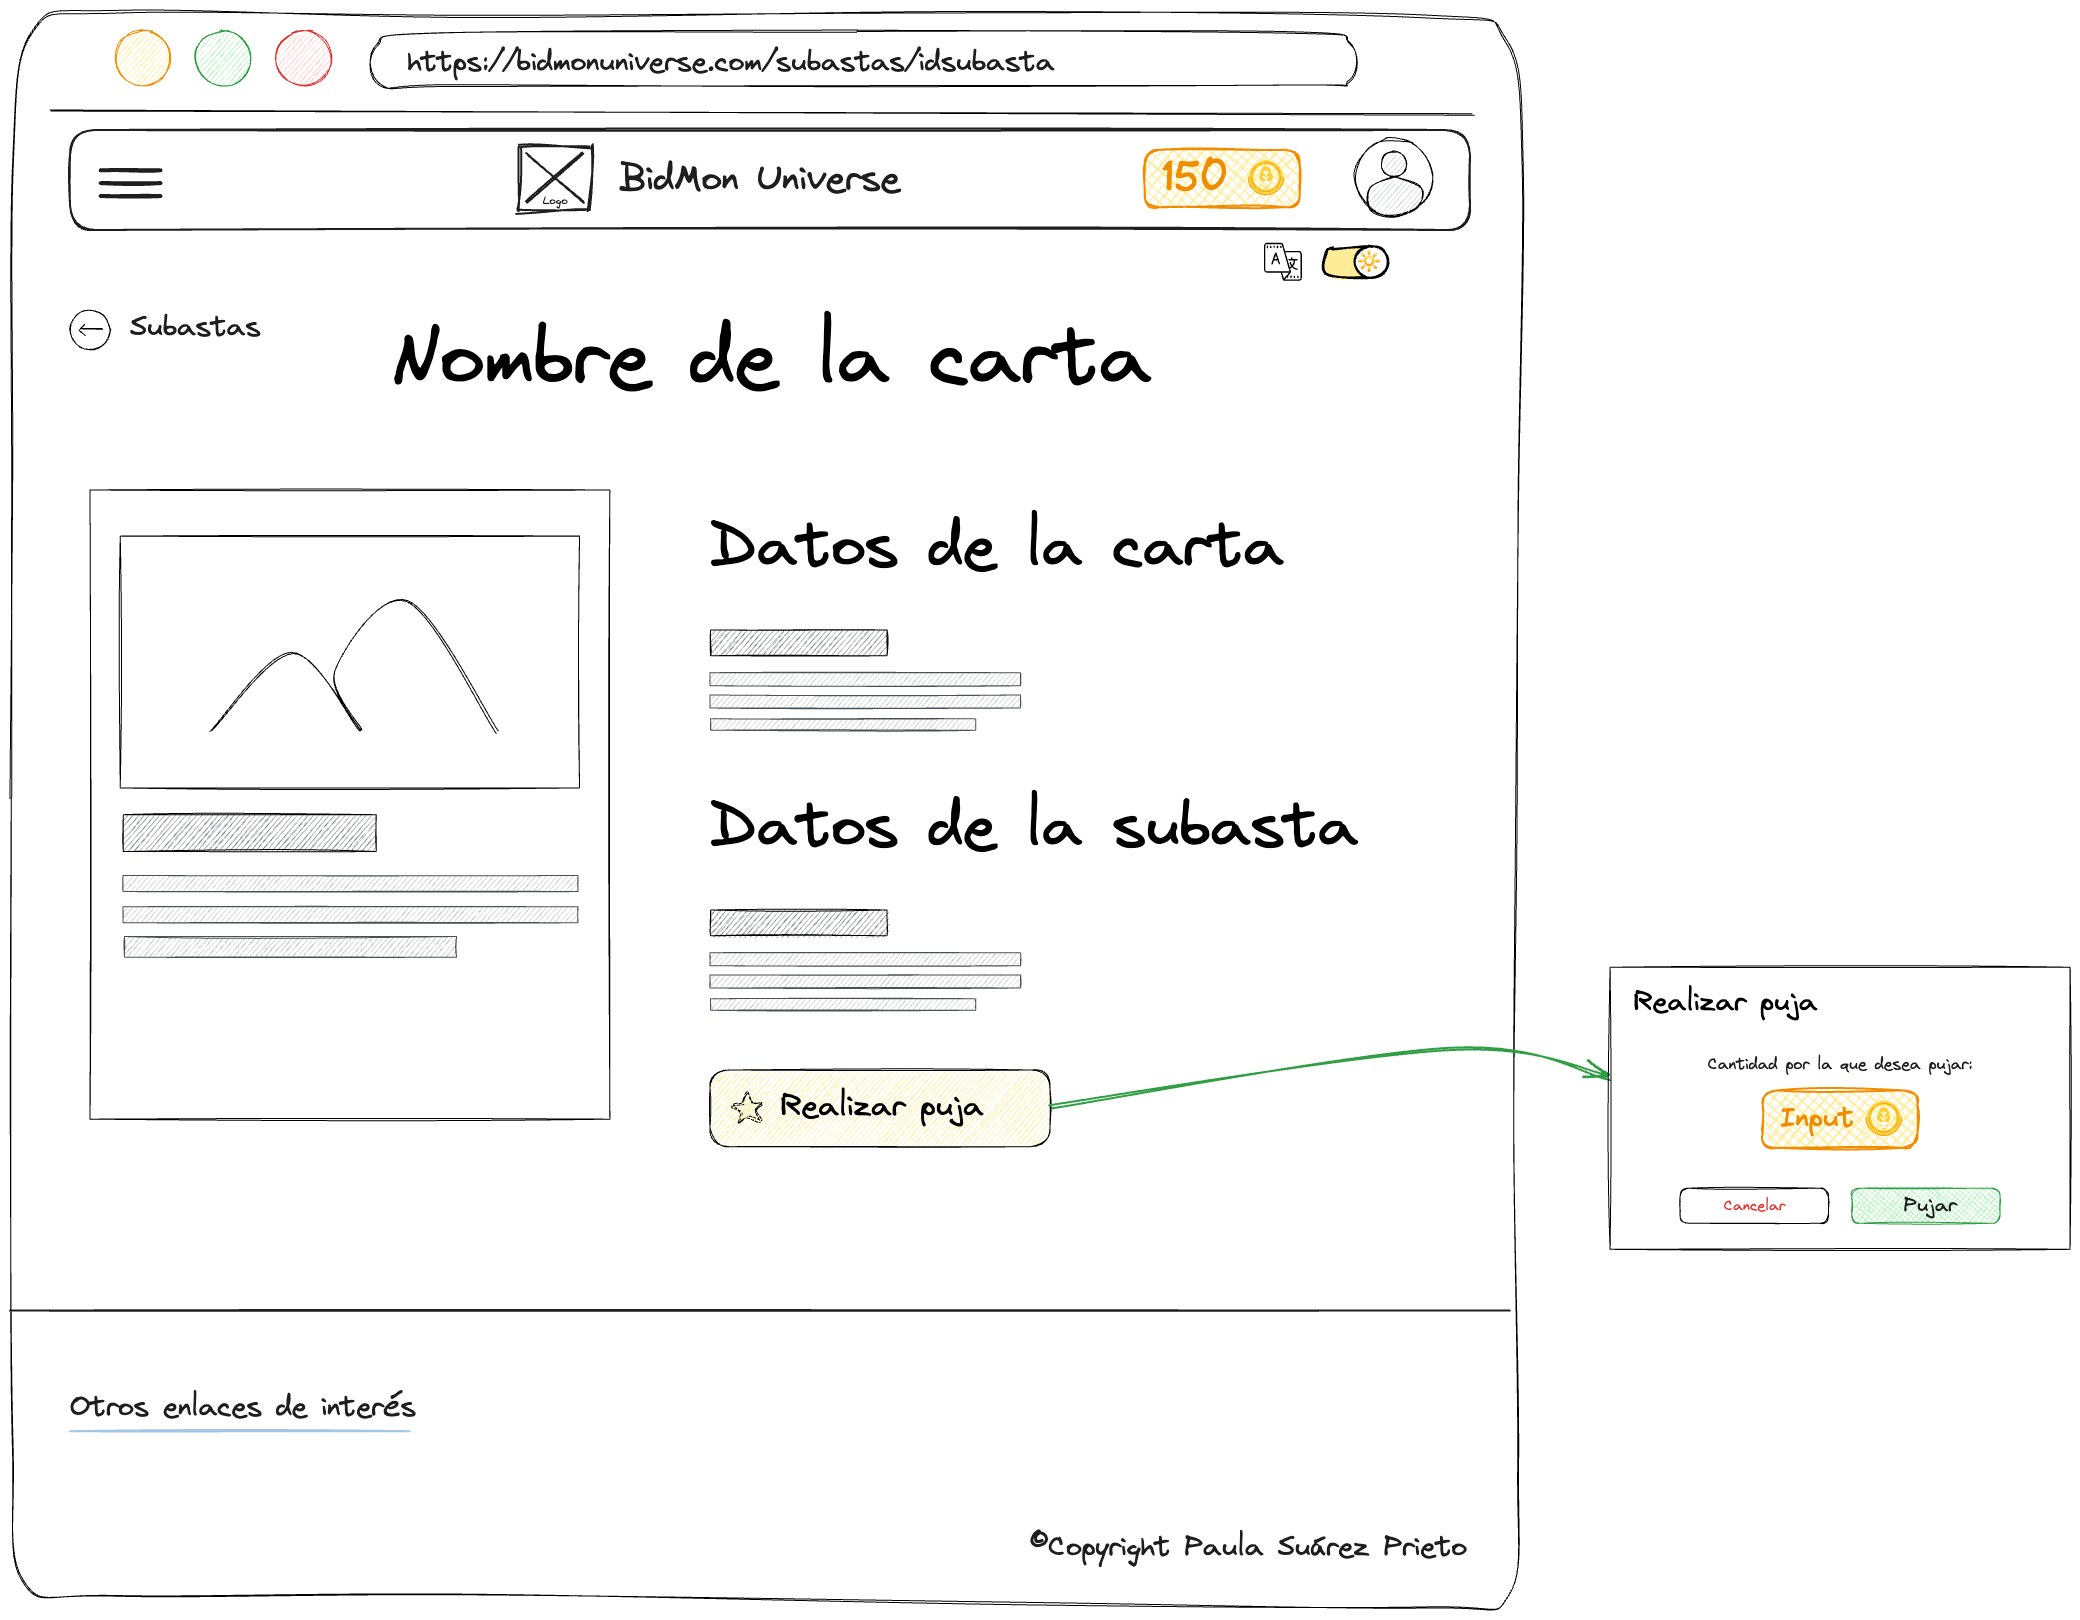
\includegraphics[width=0.9\textwidth]{figures/6-Analisis/6-Interfaz/prototipos/detalle-subasta.png}
    \caption{Boceto de la página de detalles de subasta}
    \label{fig:p_auction_details}
    \hypertarget{fig:p_auction_details}{}
\end{figure}

En el caso de que la subasta sea propia, el usuario puede cancelar la subasta como se muestra en la \coloredUnderline{\hyperlink{fig:p_auction_details_own}{Figura \ref*{fig:p_auction_details_own}: \nameref*{fig:p_auction_details_own}}}.
El usuario no puede ver las pujas recibidas en su subasta, solo puede ver la información de la subasta. Esto se debe a que el sistema implementa un sistema de pujas ciegas.
De esta manera, el dueño de la subasta no cancelará la subasta si ve que no ha recibido la puja que esperaba y los usuarios no se verán influenciados por las pujas de los demás.

\begin{figure}[H]
    \centering
    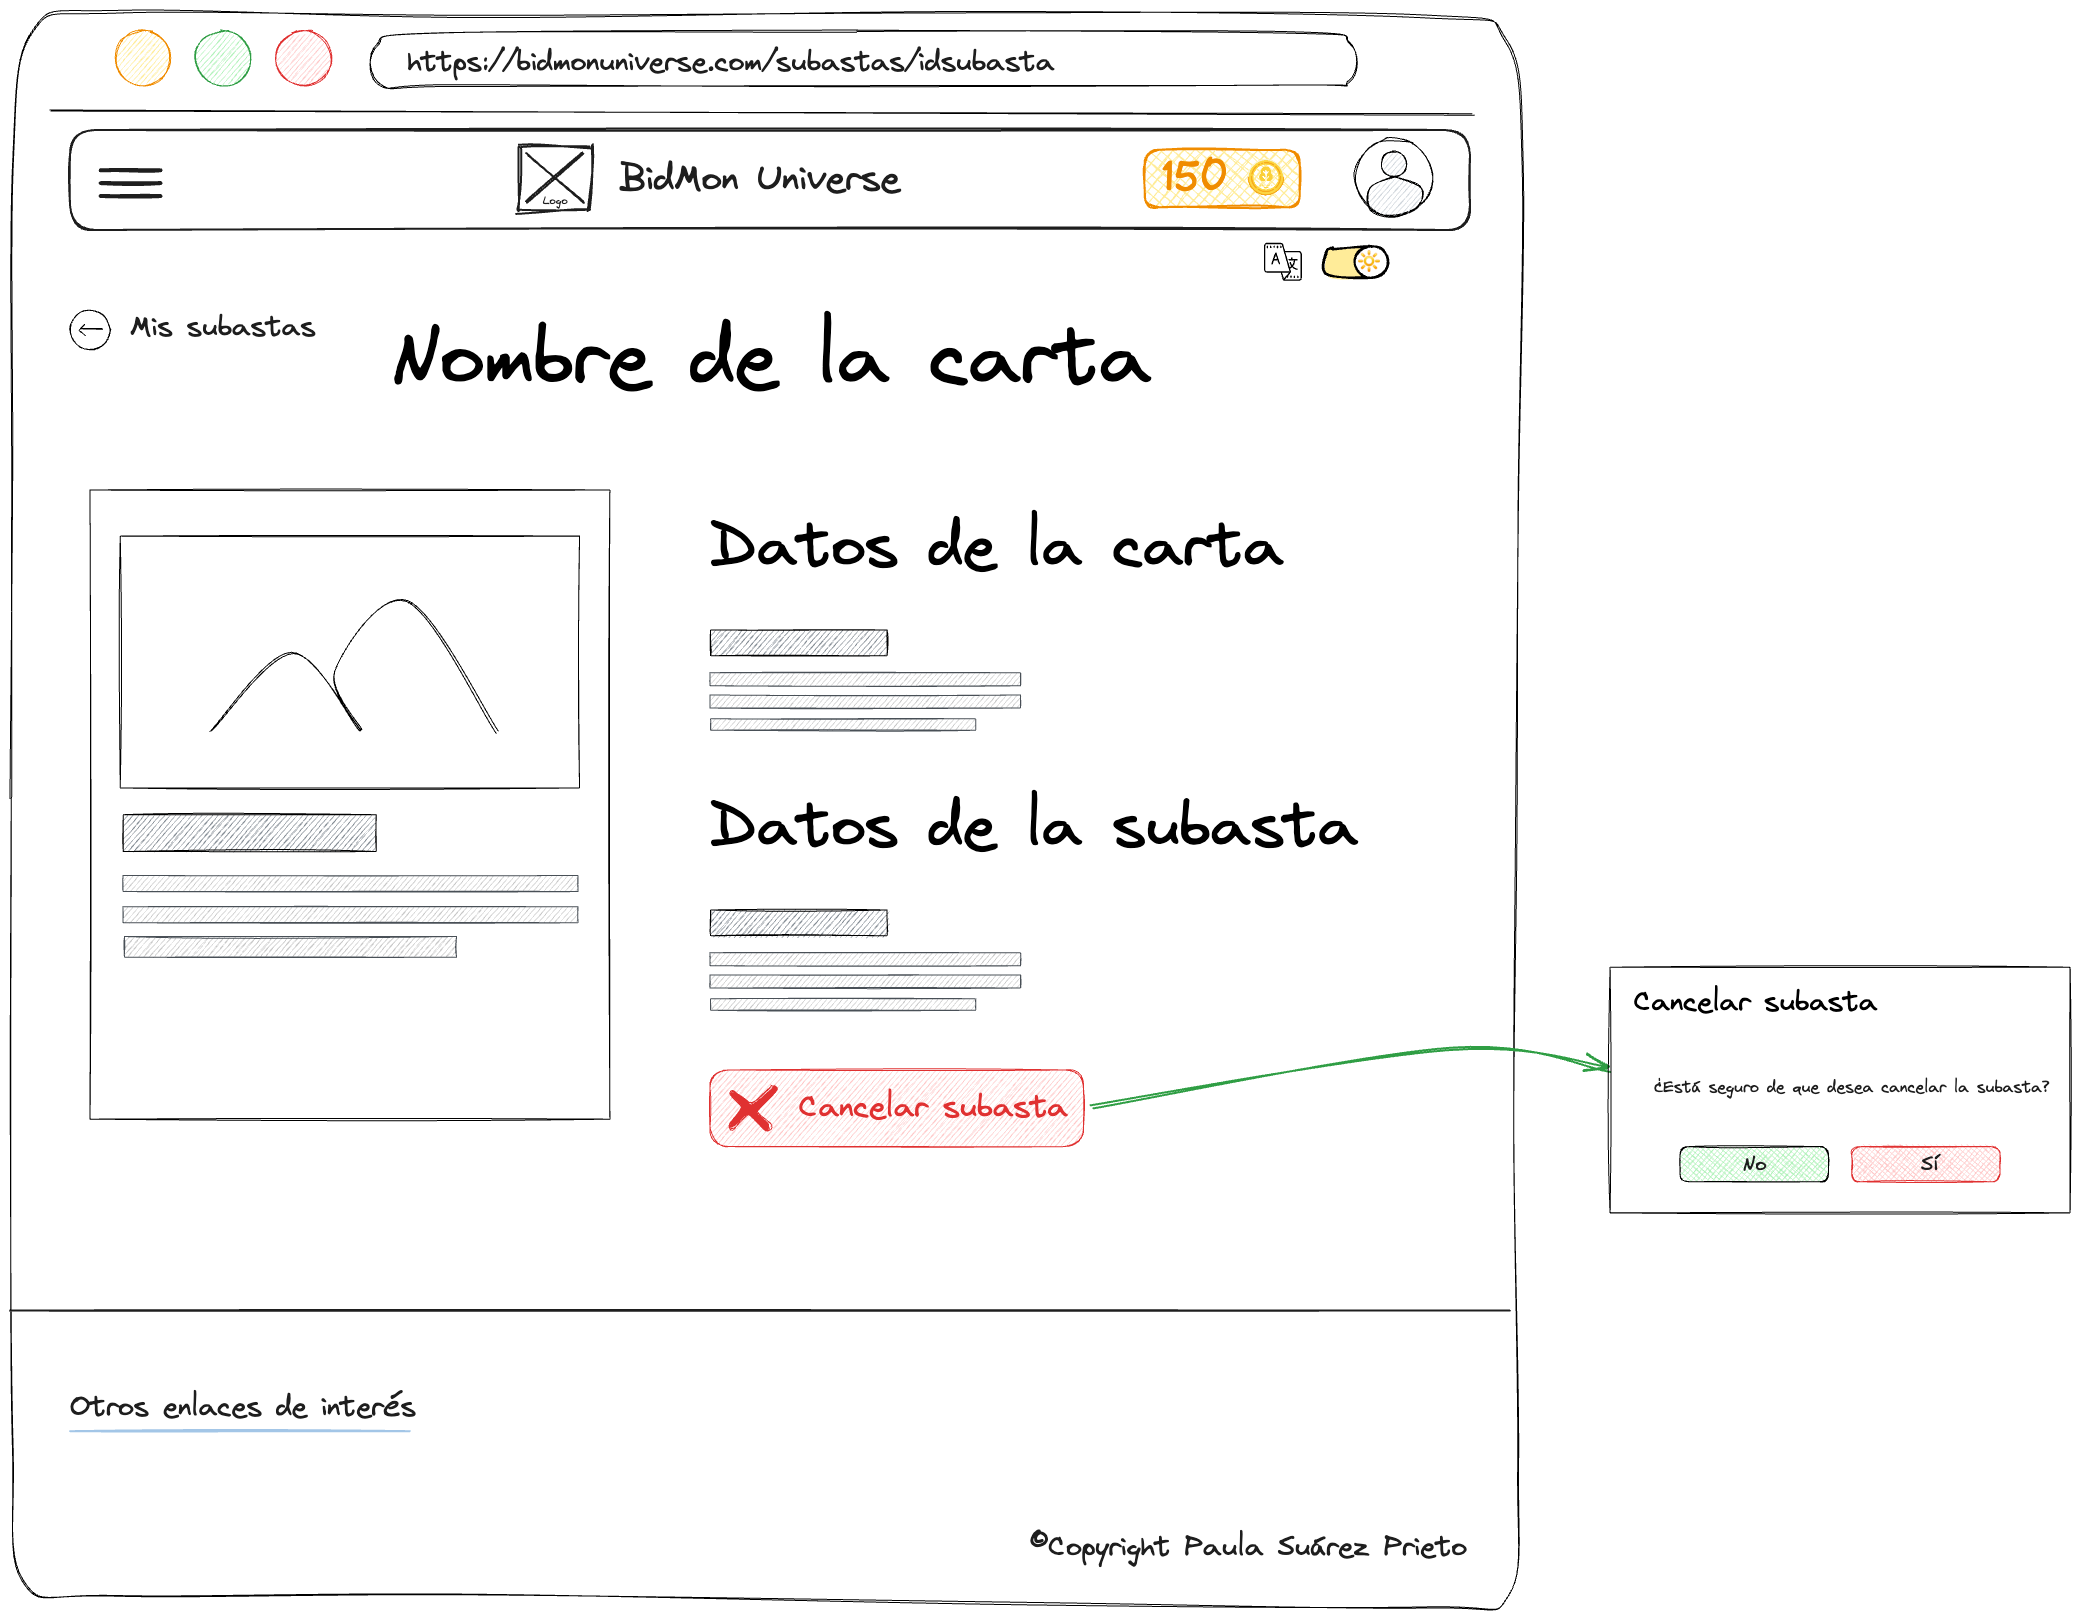
\includegraphics[width=0.9\textwidth]{figures/6-Analisis/6-Interfaz/prototipos/detalle-subasta-propia.png}
    \caption{Boceto de la página de detalles de subasta propia}
    \label{fig:p_auction_details_own}
    \hypertarget{fig:p_auction_details_own}{}
\end{figure}

En el caso de que sea una subasta en la que el usuario ha pujado, el usuario puede retirar la puja como se muestra en la \coloredUnderline{\hyperlink{fig:p_auction_details_bid}{Figura \ref*{fig:p_auction_details_bid}: \nameref*{fig:p_auction_details_bid}}}.
Por el mismo motivo que en el caso de las subastas propias, el usuario no puede ver las pujas de los demás usuarios ni la puja más alta.

\begin{figure}[H]
    \centering
    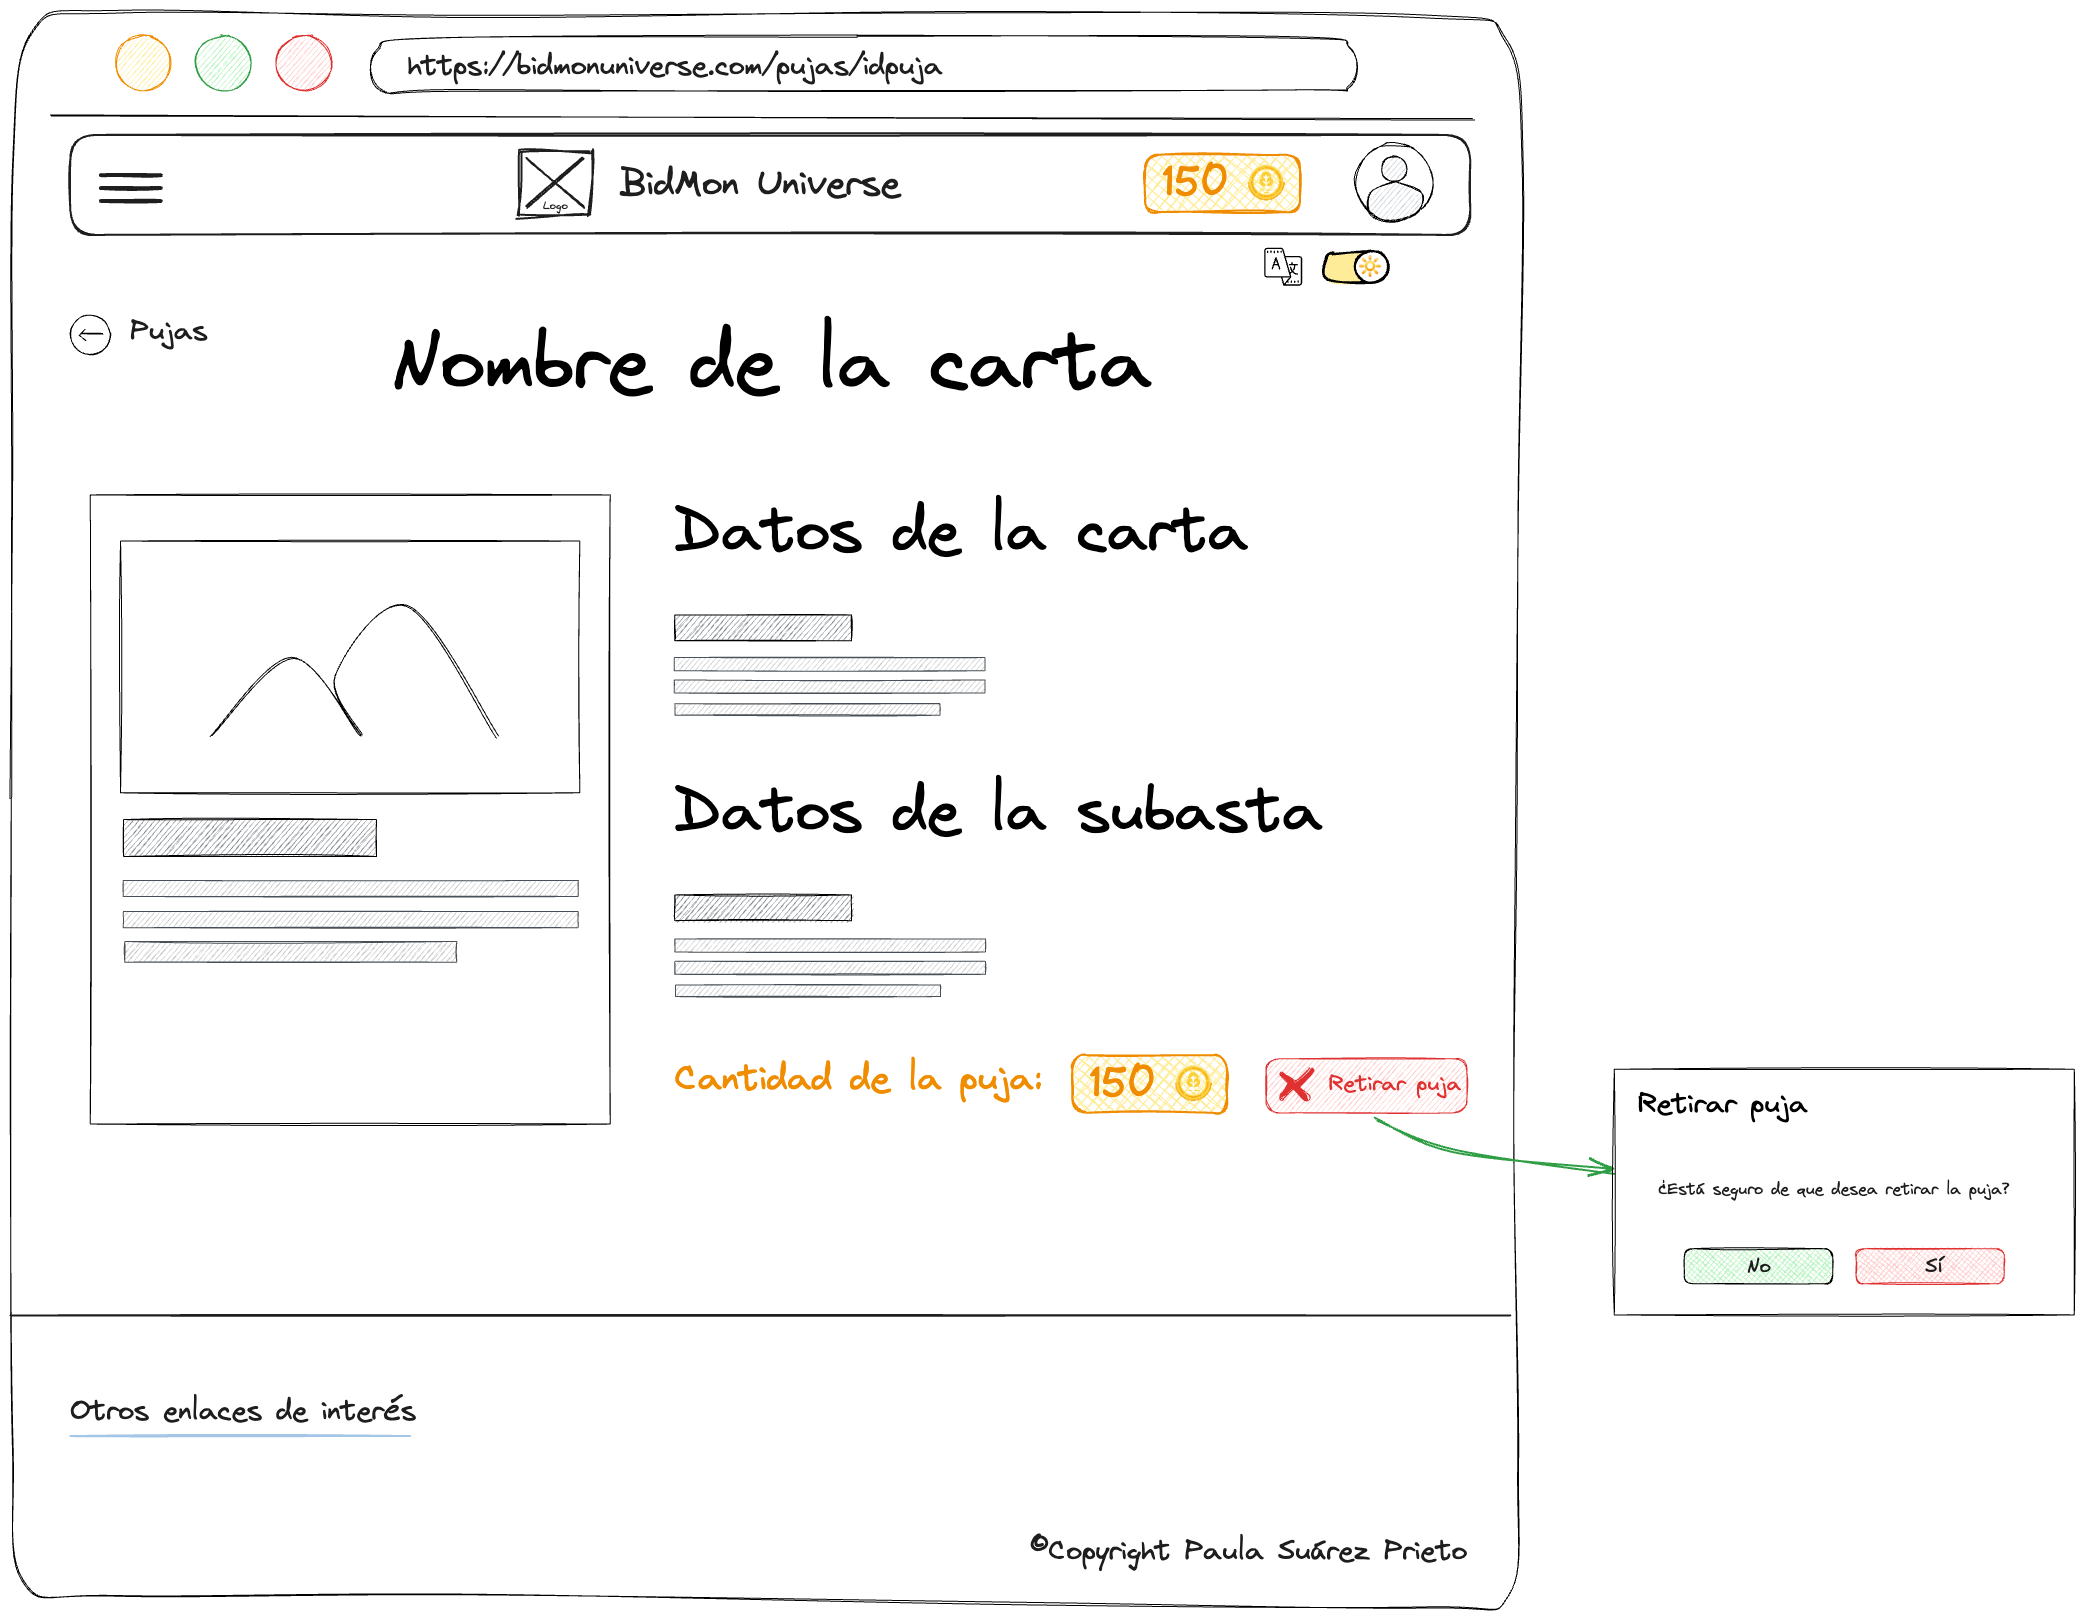
\includegraphics[width=0.9\textwidth]{figures/6-Analisis/6-Interfaz/prototipos/detalle-puja.png}
    \caption{Boceto de la página de detalles de subasta en la que el usuario ha pujado}
    \label{fig:p_auction_details_bid}
    \hypertarget{fig:p_auction_details_bid}{}
\end{figure}


\subsubsection{Página de Histórico de Transacciones}
La página de histórico de transacciones muestra una lista de las transacciones realizadas.
Si el usuario que ha iniciado sesión es un administrador, se mostrarán todas las transacciones realizadas en el sistema.
Si el usuario que ha iniciado sesión es un usuario normal, se mostrarán solo las transacciones realizadas por él.

En la \coloredUnderline{\hyperlink{fig:p_transactions}{Figura \ref*{fig:p_transactions}: \nameref*{fig:p_transactions}}}, se muestra el boceto de la página de histórico de transacciones.
\begin{figure}[H]
    \centering
    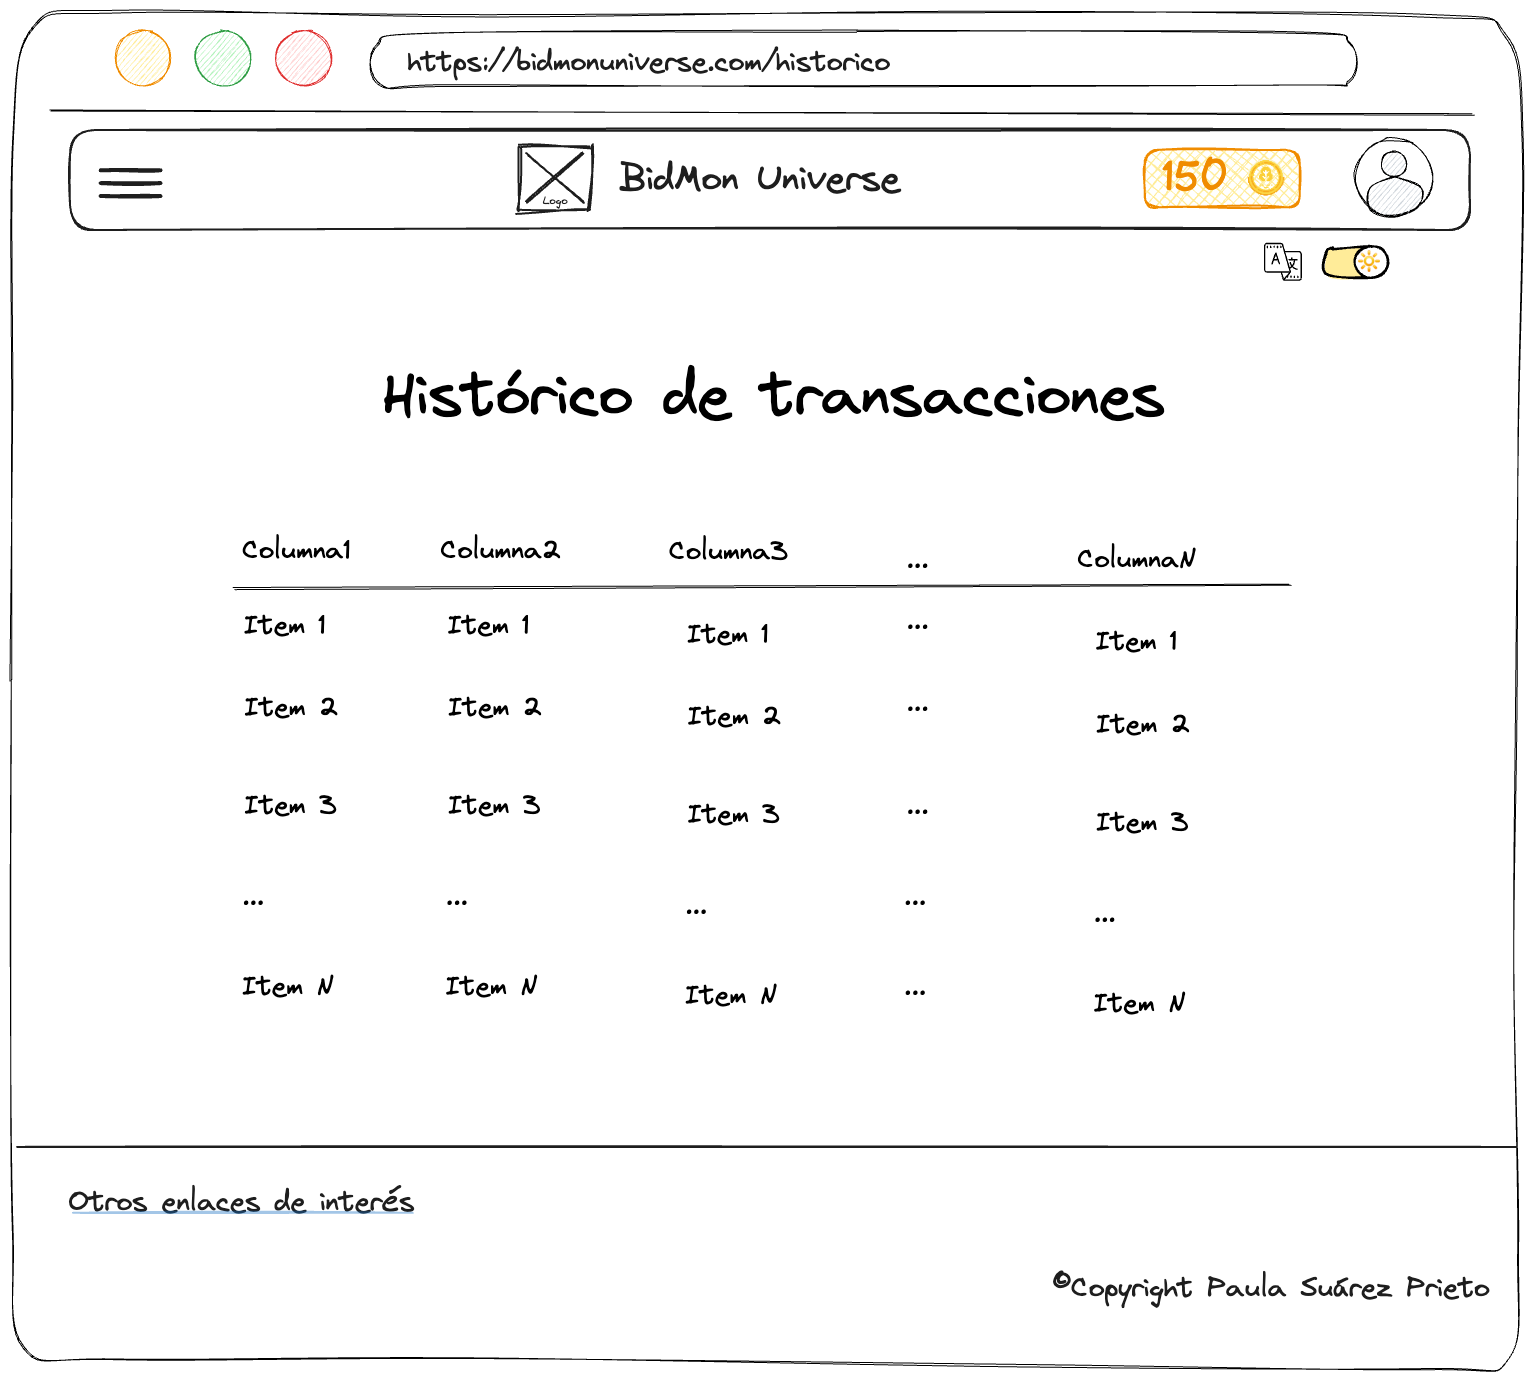
\includegraphics[width=0.9\textwidth]{figures/6-Analisis/6-Interfaz/prototipos/historico-transacciones.png}
    \caption{Boceto de la página de histórico de transacciones}
    \label{fig:p_transactions}
    \hypertarget{fig:p_transactions}{}
\end{figure}